% This is my template for presentations of diploma
% All slides in code separated by line

\documentclass[ucs,compress]{beamer}    % [ucs] makes Cyrillic fonts visible in index 
\usepackage{beamerthemeshadow}          % use <beamerthemeshadow> theme
% \usepackage{default} 			% use empty/default style, usefull for printing 
\usepackage[T2A]{fontenc}
\usepackage[utf8]{inputenc}             % set encoding
\usepackage[english,ukrainian]{babel}
\usepackage{amssymb,amsfonts,amsmath}
\usepackage{cite,enumerate,float,indentfirst}
\usepackage{graphicx,epstopdf}          % epstopdf-convert eps files to pdf
\usepackage{textcomp}

\graphicspath{{fig/},{software/}}       % look up folders for figures
\setbeamertemplate{footline}[page number] % insert number of slides
\usepackage{color}                      % you can colour your formulas with this, just use ${\color{red} E=mc^2}$
\usepackage{helvet} 	                % set font family for whole document
\usefonttheme[onlymath]{serif}          % Set font family only for math mode

\beamertemplatenavigationsymbolsempty   % hide naviagation bar

% If you want divide slide on two parts just use code:
% \begin{columns}[t]
% \begin{column}{5cm}
%  some data in column 1
% \end{column}
% \begin{column}{5cm}
%  some data in column 2
% \end{column}
% \end{columns}

% If you want to make theorem or emphasize some info, use next code:
% \begin{block}{title of block}
% Some data in block, feel free to add formulas,tables or figures here.
% \end{block} 

% use \begin{frame}[shrink=5] in case if you need insert more text in slide

\begin{document}
\title{Інтегрована інерціально-супутникова система навігації, що базується на принципах комплексної обробки інформації
з використанням калманівської фільтрації}  
% \author{доповідач:Микола Новік\\ керівник: Мар’ясова Т.І.}
\author{Доповідач: Микола Новік}
\date{\today} 
%%%%<<<<<<<<<<<<<<<<<<<<<<<<<<<<<<<<<<<<<<<<<<<<<<<<<<<<<<<<<<<<<<<<<<<<<<<<<<<<<<<
% First Slide, title page
\begin{frame}
\titlepage
\end{frame}
%%%%<<<<<<<<<<<<<<<<<<<<<<<<<<<<<<<<<<<<<<<<<<<<<<<<<<<<<<<<<<<<<<<<<<<<<<<<<<<<<<<
% Just print table of contents
% \begin{frame}[plain]
% \frametitle{Зміст доповіді}
% \tiny
% \tableofcontents
% \end{frame} 
%%%%<<<<<<<<<<<<<<<<<<<<<<<<<<<<<<<<<<<<<<<<<<<<<<<<<<<<<<<<<<<<<<<<<<<<<<<<<<<<<<<
% Intro
\section{Постановка задачі} 
\subsection{Постановка задачі та вибір системи} 
\begin{frame}\frametitle{Постановка задачі комплексування}
\small
\beamerbutton{\smallПостановка задачі}: дослідження можливостей комплексування навігаційної інформації двох систем, що є на борту сучасного літака: безплатформенної інерціальної навігаційної системи і супутникової високоточної навігаційної системи.\\
\centering \line(1,0){200}

\begin{block}<+->{В результатi комплексування IНС та СНС досягаються:}
\tiny
\begin{enumerate}
\item  пiдвищення точностi визначення координат, висоти, швидкостi i часу споживача;
\item  уточнення кутiв орiєнтацiї (курсу, крену i тангажа);
\item  оцiнка й уточнення параметрiв калiбрування навiгацiйних датчикiв,
таких, як дрейфи гiроскопiв, масштабнi коефiцiєнти, зсуви нуля акселерометрів тощо;
\item  забезпечення на цiй основi безперервностi навiгацiйних визначень на всiх етапах руху, у тому числi i при тимчасовiй непрацездатностi приймача СНС у випадках впливу завад або енергiйних маневрiв ЛА.

\end{enumerate}
\end{block}

\end{frame} 

%%%%<<<<<<<<<<<<<<<<<<<<<<<<<<<<<<<<<<<<<<<<<<<<<<<<<<<<<<<<<<<<<<<<<<<<<<<<<<<<<<<
\subsection{Вибір варіанту комплексування ІСНС } 
\begin{frame}\frametitle{Варіанти інтегрування ІСНС} 

\tiny
\begin{block}{Роздільна схема}
Надмірність, обмеженість похибок оцінок місця розташування і швидкості, 
наявність інформації про орієнтацію і кутову швидкість, висока швидкість видачі інформації, 
мінімальні зміни в бортовій апаратурі
\end{block}

\begin{exampleblock}{Слабко зв'язана схема}
Усі перераховані особливості роздільних систем, плюс більш швидке відновлення слідкування за кодом і фазою сигналів СНС, виставлення та калібрування 
БІНС у польоті, як наслідок -- підвищена точність під час відсутності сигналу СНС
\end{exampleblock}


\begin{block}{Жорстко зв'язана схема}
Подальше поліпшення точності і калібрування, підвищена стійкість слідкування 
за сигналами СНС при маневрах ЛА, підвищена завадостійкість, компактність, знижені вимоги з енергозабезпечення. Вектор стану містить до 40 компонентів, тому фільтр складно реалізувати; необхідність розробки 
спеціальних датчиків.
\end{block}
\end{frame}
%%%%<<<<<<<<<<<<<<<<<<<<<<<<<<<<<<<<<<<<<<<<<<<<<<<<<<<<<<<<<<<<<<<<<<<<<<<<<<<<<<<


\subsection{Схема комплексування ІСНС }
\begin{frame} \frametitle{Схема ІСНС} 
\begin{figure}[here]
\centering
% 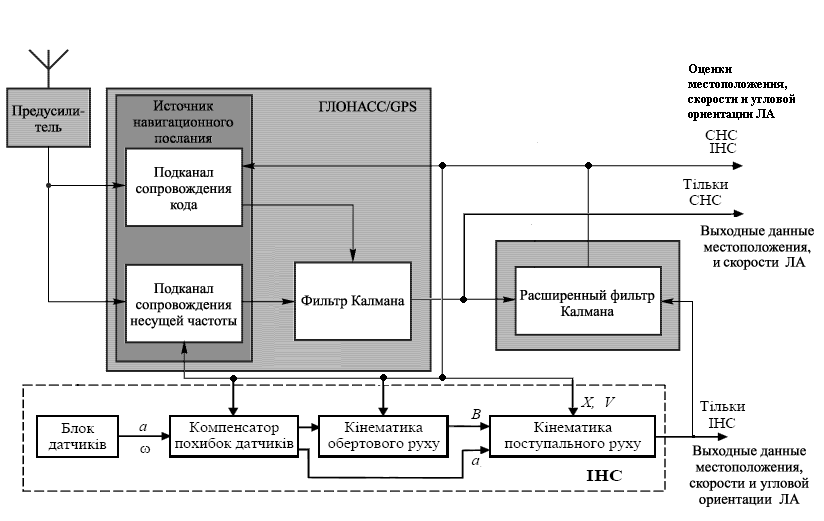
\includegraphics[width=90mm,height=65mm]{structure_scheme2}
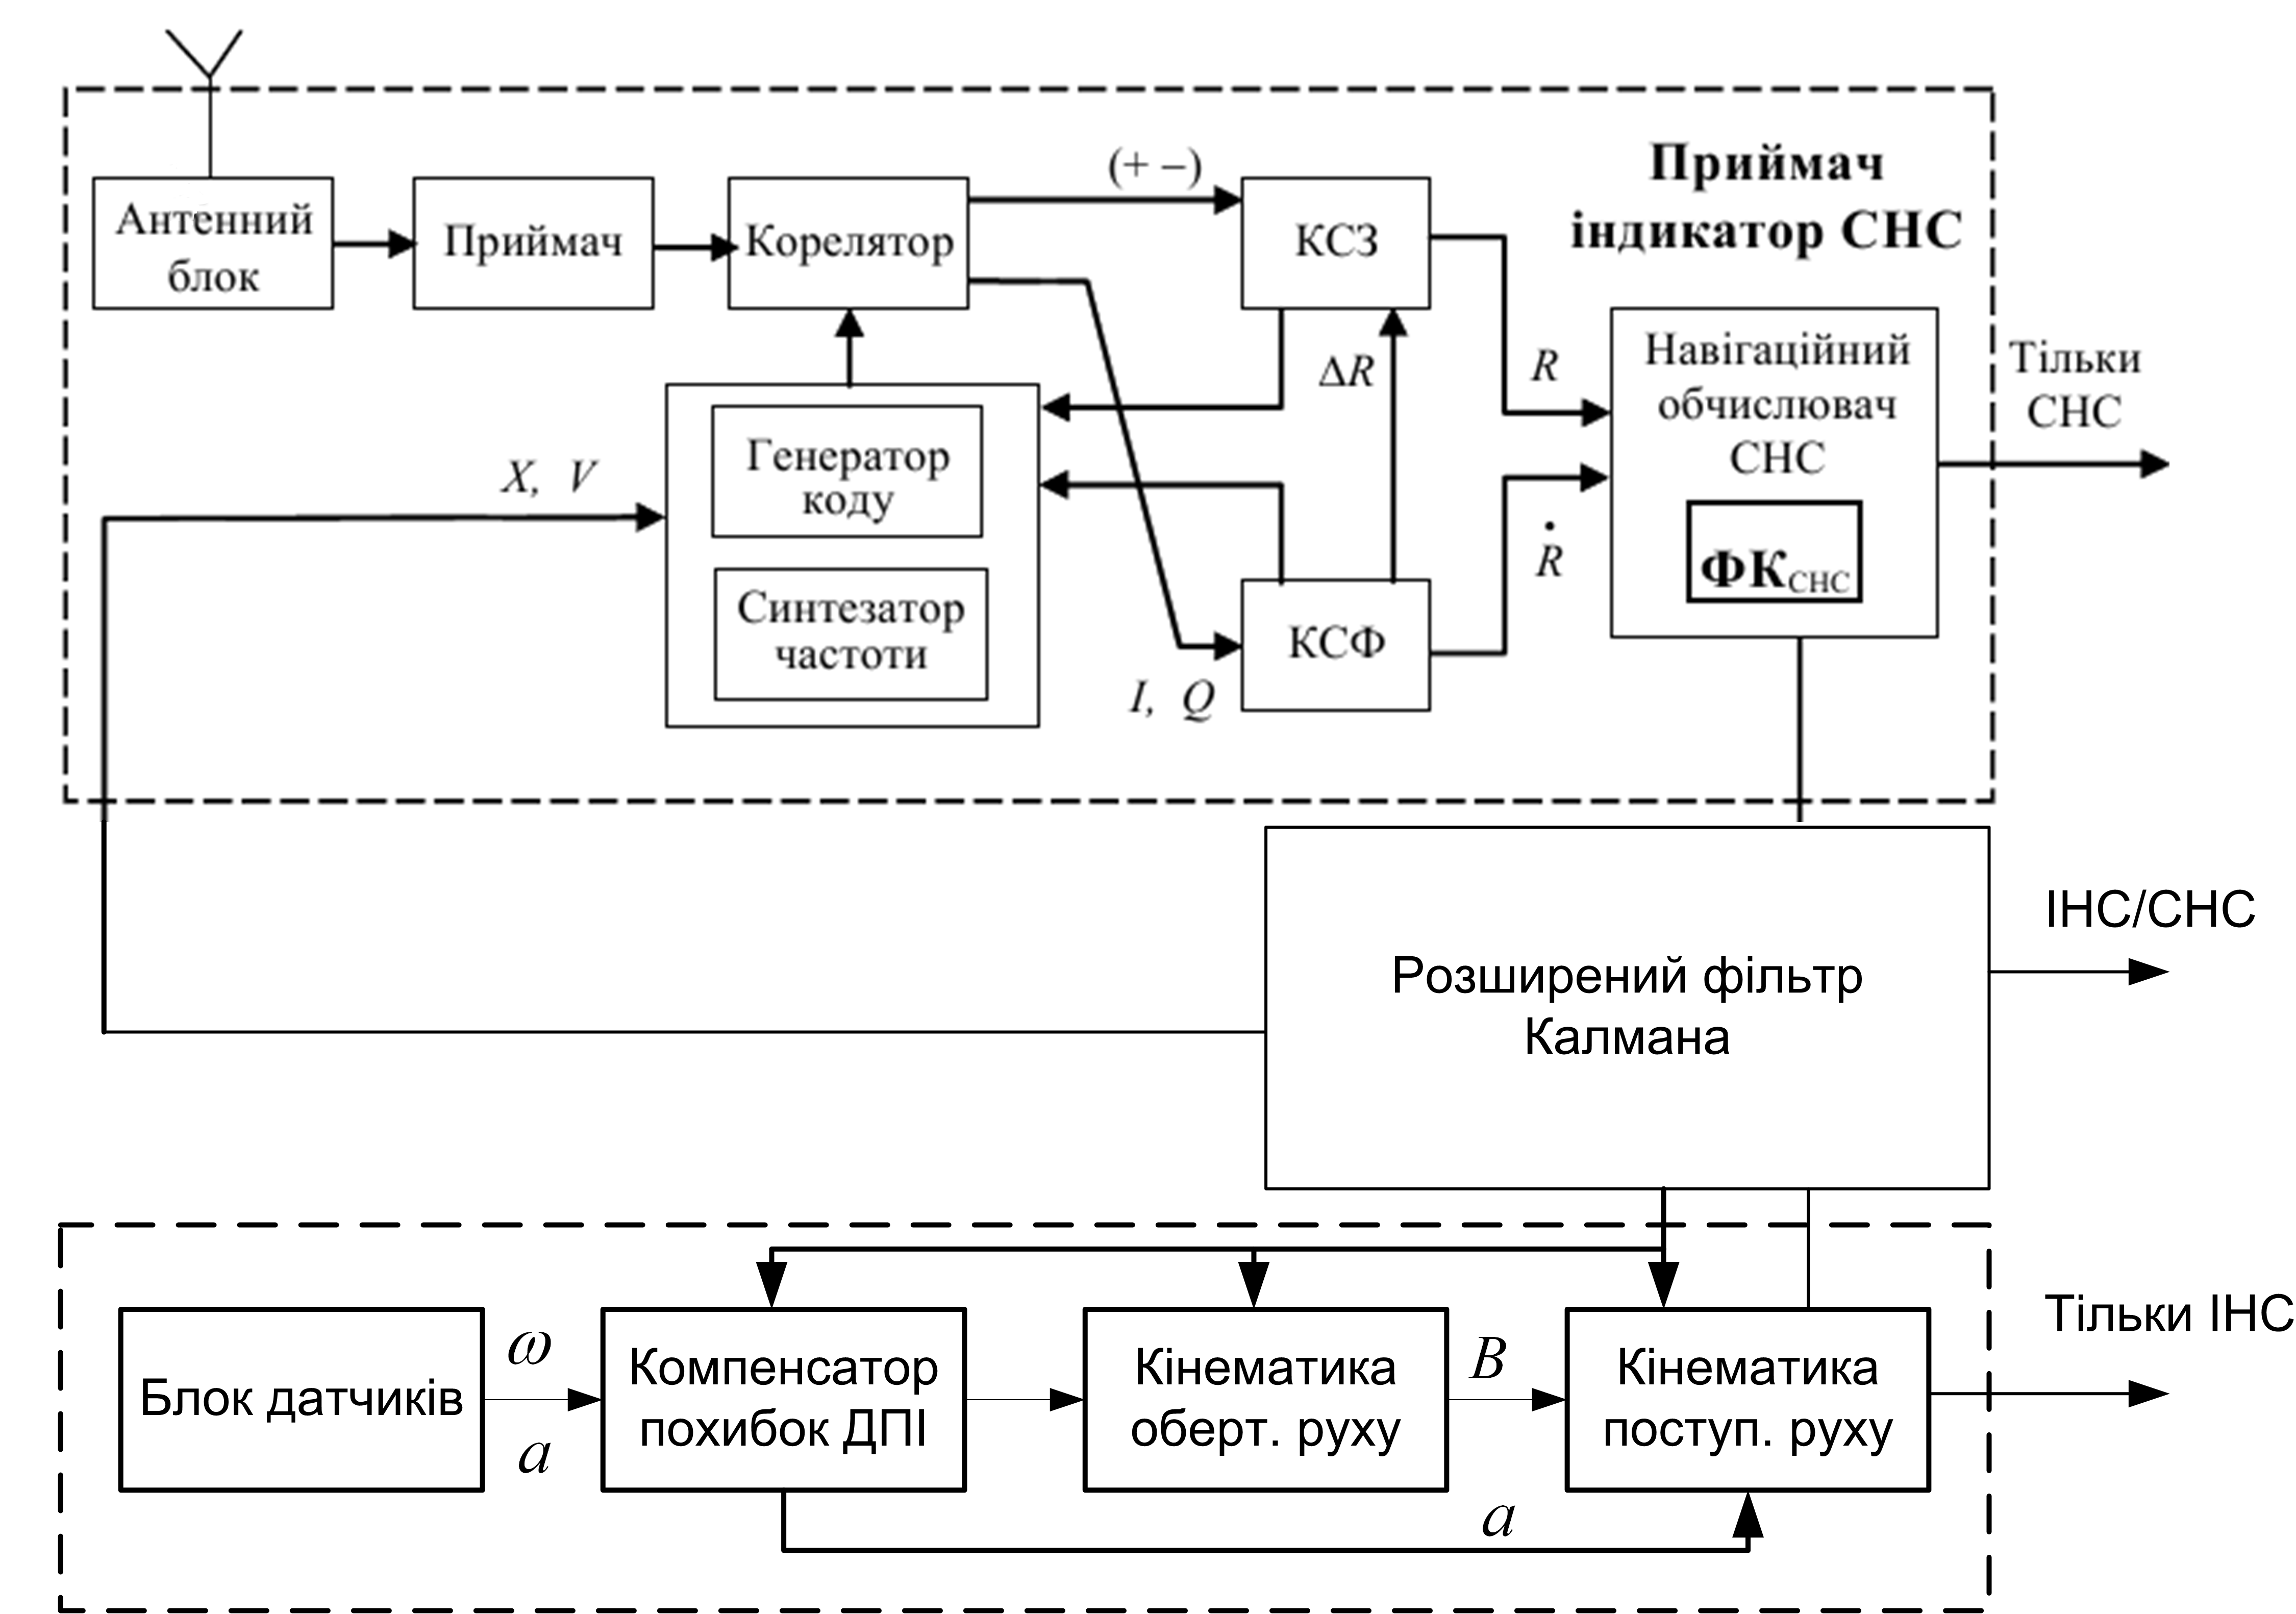
\includegraphics[scale=0.5]{sdins_main}
\caption{Слабко зв’язана схема}
%\label{fig:isns_loosly}
\end{figure}
\end{frame}

%%%%<<<<<<<<<<<<<<<<<<<<<<<<<<<<<<<<<<<<<<<<<<<<<<<<<<<<<<<<<<<<<<<<<<<<<<<<<<<<<<<


\subsection{Навігаційний Фільтр}
\begin{frame} \frametitle{Фільтр Калмана} 
\begin{figure}[here]
\centering
% 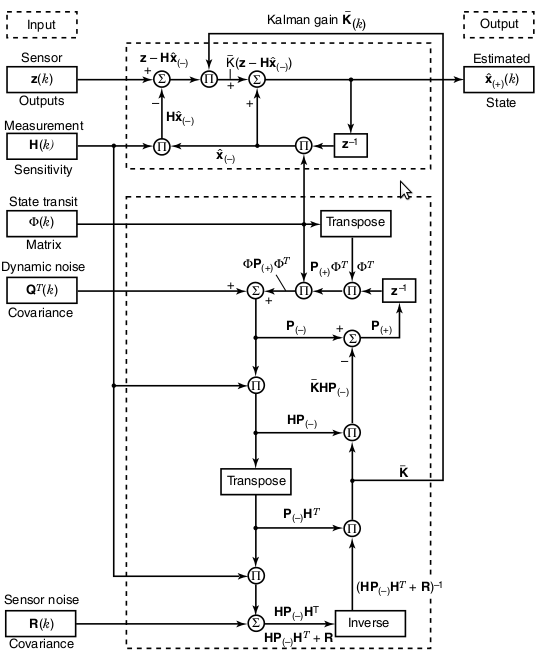
\includegraphics[width=90mm,height=65mm]{kalman_data_flow}
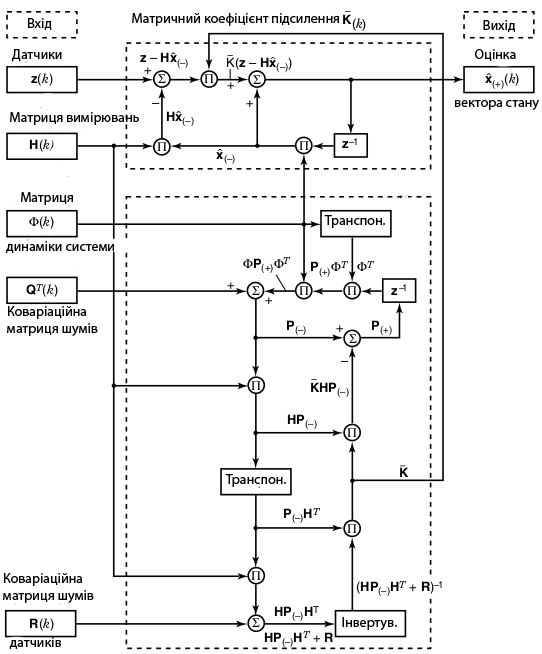
\includegraphics[scale=0.3]{kalman_data_flow2}
\caption{Схема роботи фільтра Калмана}
%\label{fig:isns_loosly}
\end{figure}
\end{frame}

%%%%<<<<<<<<<<<<<<<<<<<<<<<<<<<<<<<<<<<<<<<<<<<<<<<<<<<<<<<<<<<<<<<<<<<<<<<<<<<<<<<
\subsection{Траєкторія руху ЛА та кути крену, курса і тангажа} 
\begin{frame}[ shrink=10]
\frametitle{Траєкторія руху ЛА та кути крену, курса і тангажа}
\noindent
\begin{figure}[l]
\noindent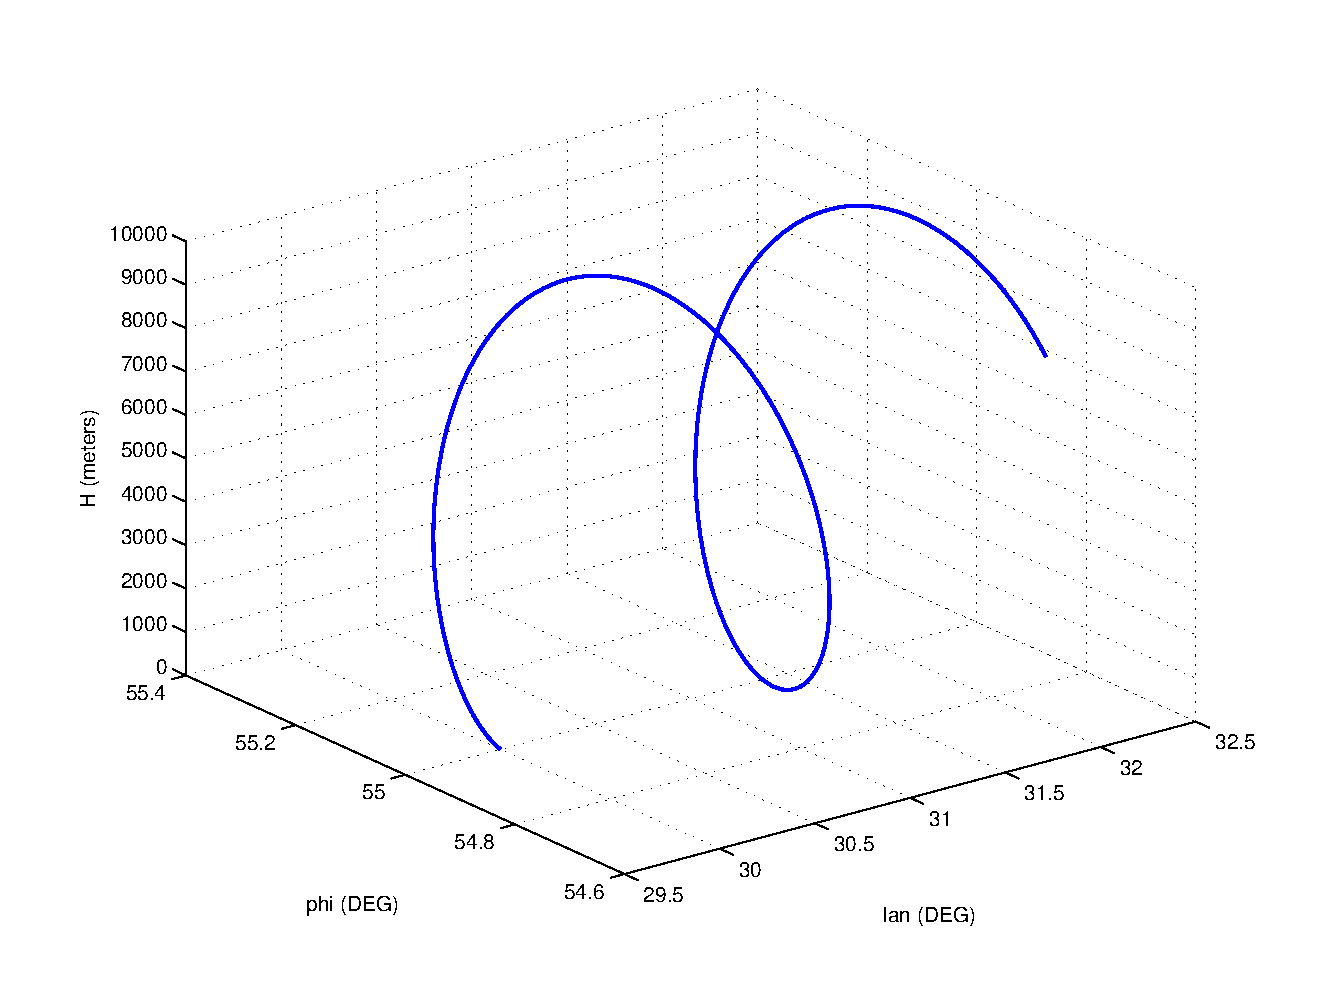
\includegraphics[scale=0.28]{path_3d}
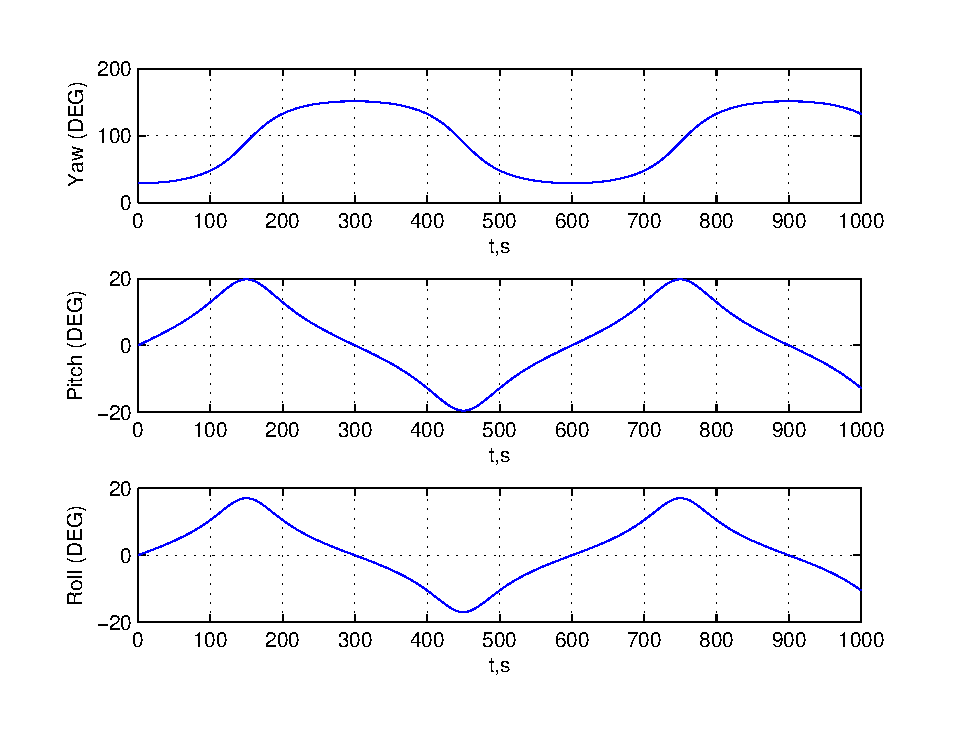
\includegraphics[scale=0.35]{path_PYR}
\caption{\tiny Траєкторія руху ЛА та його кути орієнтації }
\end{figure}\tiny
\begin{columns}[t]
\begin{column}{4cm}\noindent
$\left \{ \begin{array}{l} 
{\varphi (t)=\varphi_{0}+K_{\varphi } t+\Delta_{\varphi } \sin (\omega_{\varphi } t+\delta_{\varphi } );} \\ 
{\lambda (t)=\lambda_{0}+K_{\lambda } t+\Delta_{\lambda } \sin (\omega_{\lambda } t+\delta_{_{\lambda } } );} \\ 
{h(t)=h_{0} -\Delta h \cos (\omega_{h} t+\delta_{h} );} \\ 
\end{array}\right.$
$\left \{\begin{array}{l}
{V_{E} (t)=\dot{\lambda }(t)\left[R_{1} (\varphi )+h(t)\right]\cos \varphi (t);} \\ 
{V_{N} (t)=\dot{\varphi }(t)[R_{2} (\varphi )+h(t)];} \\ 
{V_{h} (t)=\dot{h}(t);} \\ {R_{1} (\varphi )=\frac{a}{\sqrt{1-e^{2} \sin ^{2} \varphi } } ;} \\ 
{R_{2} (\varphi )=R_{1} (\varphi )\frac{1-e^{2} }{1-e^{2} \sin ^{2} \varphi } ;} 
\end{array} \right.$
\end{column}
\begin{column}{6cm}\noindent
$\left \{\begin{array}{l} 
{a_{E}(t)=\dot{V}_{E} (t)-q(t)\sin \varphi (t)V_{N} (t)+q(t)\cos (t)V_{h} (t);} \\ 
{a_{N}(t)=\dot{V}_{N} (t)+q(t)\sin \varphi (t)V_{E} (t)+\dot{\varphi }(t)V_{h} (t);} \\ 
{a_{h}(t)=\dot{V}_{h} (t)-q(t)\cos \varphi (t)V_{E} (t)-\dot{\varphi }(t)V_{N} (t)+g(h,\varphi);} \\ 
{q(t)=\dot{\lambda }(t)+2\omega_{3} ;} \\ 
{g(h,\varphi)=g_{e} [1-2\frac{h(t)}{a} +\frac{3}{4} e^{2} \sin ^{2} \varphi (t)];} 
\end{array}\right.$
$\left \{\begin{array}{l} 
{\vartheta(t)=arctg2[V_{h} (t)/V_{r} (t)];} \\ 
{\psi (t)=arctg2[V_{E}(t)/V_{N} (t)];} \\ 
{\gamma (t)=K_{\gamma }\frac{V_{N}(t)\dot{V}_{E}(t)-V_{E}(t)\dot{V}_{N}(t)}{V_{r}(t)\cos v(t)},}
 \end{array}\right.$
\end{column}
\end{columns}
\end{frame}
%%%%<<<<<<<<<<<<<<<<<<<<<<<<<<<<<<<<<<<<<<<<<<<<<<<<<<<<<<<<<<<<<<<<<<<<<<<<<<<<<<<

\section{Модель системи }
\subsection{Алгоритми роботи БІНС}

 
\begin{frame}
\frametitle{Алгоритми роботи БІНС}

\begin{figure}[here]
\centering
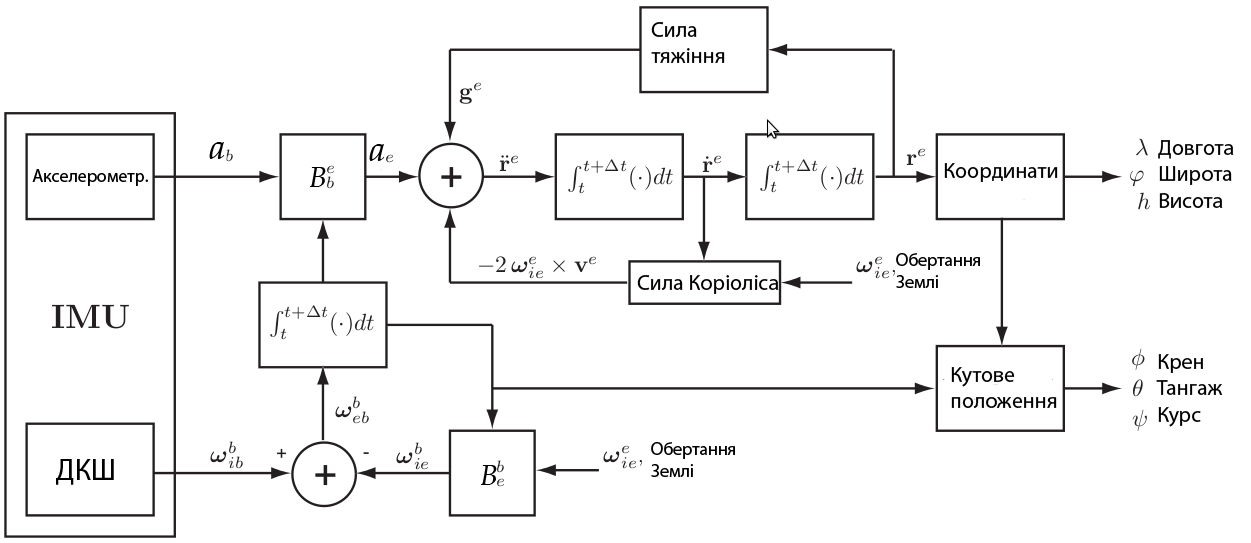
\includegraphics[scale=0.2]{sdins_algorithm2}
\end{figure}
\tiny

\begin{columns}[t]
\begin{column}{5cm}
\beamerbutton{Координати}\\
$\left\{ \begin{array}{l} 
{\dot{\lambda }=\frac{V_{E} \left(t\right)}{\left(R_{1} +h\right)\cos \varphi \left(t\right)} } \\ 
{\dot{\varphi }=\frac{V_{N} \left(t\right)}{\left(R_{2} +h\right)} } \\ 
{\dot{h}=V_{h} \left(t\right)} \end{array}\right .$    \\ 

\end{column}
\begin{column}{5cm}
 \beamerbutton{Швидкості}\\
$\dot{\bar{V}}=B\bar{a}{}_{c} -\Delta \bar{n}\left(t\right)+\bar{g}_{T} $\\
\beamerbutton{Орієнтація}\\
$\dot{B}=B\Omega _{c} -\Omega _{\Gamma } B$\\
\end{column}
\end{columns}

Матриця орієнтації:\\
$B%(\psi ,\vartheta ,\gamma )
=\left[\begin{array}{ccc} 
{\sin \psi \cos \vartheta } & {\cos \psi \sin \gamma -\sin \psi \cos \gamma \sin \vartheta } & {\cos \psi \cos 
\gamma +\sin \psi \sin \gamma \sin \vartheta } \\ 
{\cos \psi \cos \vartheta } & {-\sin \psi \sin \gamma -\cos \psi \cos \gamma \sin \vartheta } & {-\sin \psi \cos \gamma +\cos \psi \sin \gamma \sin \vartheta } \\ 
{\sin \vartheta } & {\cos \gamma \cos \vartheta } & {-\sin \gamma \cos \vartheta } \end{array}\right]$


% \end{block}

% $\Omega_{c} =\left[\begin{array}{ccc} 
% {0} & {-\omega_{z1} } & {\omega_{y1} } \\ 
% {\omega_{z1} } & {0} & {-\omega_{x1} } \\ 
% {-\omega_{y1} } & {\omega_{x1}} & {0} 
% \end{array}\right]$ $\Omega _{\Gamma } =\left[\begin{array}{ccc} 
% {0} & {-\left(\dot{\lambda }+u\right)\sin \varphi } & {\left(\dot{\lambda }+u\right)\cos \varphi } \\ {\left(\dot{\lambda }+u\right)\sin \varphi } & {0} & {\dot{\varphi }} \\ 
% {-\left(\dot{\lambda }+u\right)\cos \varphi } & {-\dot{\varphi }} & {0} 
% \end{array}\right]$ 
% 
% Вектор проекцій суми переносного и кориолісова прискорень на осі гео-графічної СК
% $\begin{array}{l} 
% {\Delta n_{E} =\frac{V_{E} V_{h} }{R_{1} +h} -\frac{V_{E} V_{N} }{R_{1} +h} tg\varphi +2u\left(V_{h} \cos \varphi -V_{N} \sin \varphi \right);} \\ 
% {\Delta n_{N} =\frac{V_{N} V_{h} }{R_{2} +h} +\frac{V_{E}^{2} }{R_{1} +h} tg\varphi +2uV_{E} \sin \varphi ;} \\ {\Delta n_{h} =-\frac{V_{E}^{2} }{R_{1} +h} -\frac{V_{N}^{2} }{R_{2} +h} -2uV_{E} \cos \varphi ;} 
% \end{array}$



% Головні радіуси кривизни обраного земного еліпсоїда:\\
% $\begin{array}{l} 
% {R_{1} =a\left[1-e^{2} \sin ^{2} \varphi (t)\right]^{-\frac{1}{2}};} \\ 
% {R_{2} =a\left(1-e^{2} \right)\left[1-e^{2} \sin ^{2} \varphi (t)\right]^{- \frac{3}{2} } ;} 
% \end{array}$
\end{frame}

%%%%<<<<<<<<<<<<<<<<<<<<<<<<<<<<<<<<<<<<<<<<<<<<<<<<<<<<<<<<<<<<<<<<<<<<<<<<<<<<<<<
\subsection{Рівняння похибок БІНС} 
\begin{frame}[ shrink=10]
\frametitle{Рівняння похибок БІНС}
\begin{block}{БІНС}
\tiny
Похибка приведеної координати:\\
$\begin{array}{l} 
{\Delta \dot{R}_{E} =\Delta V_{E}(t)\cdot \frac{R_{\text{З}} }{R\cos \varphi (t)} 
+\Delta R_{N} (t)\frac{V_{E}^{}(t)\sin \varphi (t)}{R_{\text{З}} R\cos ^{2} \varphi (t)} 
-\Delta h(t)\frac{R_{\text{З}} V_{E}^{}(t)}{R^{2} \cos \varphi (t)} ;} \\ 
{\Delta \dot{R}_{N} =\Delta V_{N}(t)\cdot \frac{R_{\text{З}}}{R} -\Delta h(t)\frac{R_{\text{З}} V_{N}(t)}{R^{2}};} \\ 
{\Delta \dot{h} =\Delta V_{h} (t);} \end{array} $

{\centering \line(1,0){300}\\}
Похибка швидкості:\\
$\begin{array}{l}{\Delta \dot{V}_{E} =a_{N} \alpha_{h} -a_{h} \alpha_{N} +\sum_{i=1}^{3}b_{1,i}  \Delta a_{i} -\Delta V_{h} U(t)\cos \varphi +\Delta V_{N}U(t)\sin \varphi +} \\ 
{+\frac{\Delta R_{N} }{R_{\text{З}} } \left(U(t)(V_{h} \sin \varphi +V_{N}\cos \varphi \right))-(\frac{\Delta V_{E} }{R\cos \varphi } +\frac{V_{E} \sin \varphi}{R\cos ^{2} \varphi } \frac{\Delta R_{N} }{R_{\text{З}} } )\times } \\ 
{\times (V_{h} \cos \varphi -V_{N} \sin \varphi )+\frac{\Delta hV_{E} }{R^{2} } (V_{h} -V_{N}tg\varphi);} \\
\\
{\Delta \dot{V}_{N} =-a_{E}\alpha_{h} +a_{h} \alpha_{E} +\sum_{i=1}^{3}b_{2,i}  \Delta a_{i} -\Delta V_{E}U(t)\sin \varphi -\Delta V_{h} \dot{\varphi }(t)-} \\ 
{-\frac{\Delta R_{N} }{R_{\text{З}}} V_{E} U(t)\cos \varphi -\frac{\Delta V_{N} }{R} V_{h} -(\frac{\Delta V_{E} }{R\cos \varphi } +\frac{V_{E} \sin \varphi }{R\cos ^{2} \varphi } \frac{\Delta R_{N} }{R_{\text{З}} } )V_{E} \sin \varphi +} \\ 
{+\frac{\Delta h}{R^{2} } (V_{E}^{2} tg\varphi +V_{N} V_{h} );} \\
\\
{\Delta \dot{V}_{h} =a_{E} \alpha_{N} -a_{N} \alpha_{E} +\sum_{i=1}^{3}b_{3,i}  \Delta a_{i} +\Delta V_{E} U(t)\cos \varphi +\Delta V_{N} \dot{\varphi }(t)-} \\ 
{-\frac{\Delta R_{N} }{R_{\text{З}} } V_{E} U(t)\sin \varphi +\frac{\Delta V_{N} }{R} V_{N} +(\frac{\Delta V_{E} }{R\cos \varphi } +\frac{V_{E} \sin \varphi }{R\cos ^{2} \varphi } \frac{\Delta R_{N} }{R_{\text{З}} } )V_{E} \cos \varphi +} \\ 
{+g_{e} \left(-\frac{2\Delta h}{a} +\frac{3}{2} e^{2} \sin \varphi \cos \varphi \frac{\Delta R_{N} }{R_{\text{З}} } \right)-\frac{\Delta h}{R^{2} } \left(V_{E}^{2} +V_{N}^{2} \right),} 
\end{array}\label{eq:dVsdins}$

{\centering \line(1,0){300}\\}
Похибка орієнтації координатного тригранника:\\
$\label{eq:dasdins} \begin{array}{l} 
{\dot{\alpha }_{E} =-\omega_{N} \alpha_{h} +\omega_{h} \alpha_{N} -\frac{\Delta V_{N} }{R} -\sum_{i=1}^{3}b_{1,i}\varepsilon_{i} ,} \\
{\dot{\alpha }_{N} =-\omega_{h} \alpha_{E} +\omega_{E} \alpha_{h} +\frac{\Delta V_{E} }{R} -u\sin \varphi \frac{\Delta R_{N} }{R_{\text{З}} }
-\sum_{i=1}^{3}b_{2,i}  \varepsilon_{i} ,} \\ 
{\dot{\alpha }_{h} =-\omega_{E} \alpha_{N} +\omega_{N} \alpha_{E} +\frac{\Delta V_{E} }{R} tg\varphi +(u\cos \varphi +\frac{V_{E} }{R\cos ^{2} \varphi } )
\frac{\Delta R_{N} }{R_{\text{З}} } -\sum_{i=1}^{3}b_{3,i}\varepsilon_{i} ,} \end{array} $
\end{block}
\end{frame}

%%%%<<<<<<<<<<<<<<<<<<<<<<<<<<<<<<<<<<<<<<<<<<<<<<<<<<<<<<<<<<<<<<<<<<<<<<<<<<<<<<<
\subsection{Матриця динаміки БІНС} 
\begin{frame}[ shrink=10]
\frametitle{Матриця динаміки БІНС}
\small
% F_{p,k}
\[F_{p,k} = \left[\begin{array}{cccc cc}
% {1} & {2} & {3} & {4} & {5} & {6} & {7} & {8} & {9} & {0} & {1} & {2} & {3} & {4} & {5}\\ 
% Position
{.} & {\frac{\dot{\lambda }}{R_{\text{З}} } tg\varphi;} & {\frac{-\dot{\lambda }R_{\text{З}} }{R}} & {\frac{R_{\text{З}} }{R\cos \varphi }} & {.} & {.} \\
{.} & {.} & {\frac{-\dot{\varphi }R_{\text{З}} }{R}} & {.} & {\frac{R_{\text{З}} }{R}} & {.} \\
{.} & {.} & {.} & {.} & {.} & {1} \\
% Velocity
{.} & {\begin{array}{c}{\frac{2u+\dot{\lambda }}{R_{\text{З}} } \left(V_{h} \sin \varphi  +V_{N} \cos \varphi \right)}\\
{-\frac{\dot{\lambda }}{R_{\text{З}} } tg\varphi \left(V_{h} \cos \varphi -V_{N} \sin \varphi \right)}\end{array}} & 
{\frac{V_{E} }{R^{2} } \left(V_{h} -V_{N} tg\varphi \right)} & 
{\frac{V_{N}\sin \varphi -V_{h} \cos \varphi }{R\cos \varphi }} & 
{\left(2u+\dot{\lambda }\right)\sin \varphi} & 
{-\left(2u+\dot{\lambda }\right)\cos \varphi} \\ 

{.} & {-\frac{2u+\dot{\lambda }}{R_{\text{З}} }V_{E} \cos \varphi -\frac{V_{E}^{2} }{RR_{\text{З}} } tg^{2} \varphi} & 
{\frac{V_{E}^{2} tg\varphi +V_{h} V_{N} }{R^{2} }} & 
{-\left(2u+\dot{\lambda }\right)\sin \varphi;} & 
{-\frac{V_{h} }{R}} & 
{-\dot{\varphi }(t)} \\ 

{.} & {-2u\frac{V_{E}^{} \sin \varphi }{R} +\frac{3g_{e} }{2R_{\text{З}}} e^{2} \sin \varphi \cos \varphi} & 
{-\frac{2g_{e} }{a} -\frac{V_{E}^{2} +V_{N}^{2}}{R^{2}}} & 
{\left(2u+\dot{\lambda }\right)\cos \varphi} & 
{\dot{\varphi }(t)+\frac{V_{N} }{R}} & {.} \\
 

% Alpha
{.} & {.} & {.} & {.} & {-\frac{1}{R}} & {.} \\ 
{.} & {-\frac{u}{R} \sin \varphi} & {.} & {\frac{1}{R}} & {.} & {.} \\ 
{.} & {\frac{1}{R}_{\text{З}} (u\cos \varphi +\frac{\dot{\lambda }}{\cos \varphi })} & {.} & {\frac{tg\varphi }{R}} & {.} & {.} \\ 

% othe staff
{.} & {.} & {.} & {.} & {.} & {.} \\
{.} & {.} & {.} & {.} & {.} & {.} \\
{.} & {.} & {.} & {.} & {.} & {.} \\ 
{.} & {.} & {.} & {.} & {.} & {.} \\
{.} & {.} & {.} & {.} & {.} & {.} \\
{.} & {.} & {.} & {.} & {.} & {.} \\
\end{array}\right. \] 


\[\left. \begin{array}{cccc cccc cccc cc}
% {1} & {2} & {3} & {4} & {5} & {6} & {7} & {8} & {9} & {0} & {1} & {2} & {3} & {4} & {5}\\ 
% Position
{.} & {.} & {.} & {.} & {.} & {.} & {.} & {.} & {.}\\ 
{.} & {.} & {.} & {.} & {.} & {.} & {.} & {.} & {.}\\ 
{.} & {.} & {.} & {.} & {.} & {.} & {.} & {.} & {.}\\ 

{.} & {-a_{h}} & {a_{N}} & {.} & {.} & {.} & 
{b_{1,1}} & {b_{1,2}} & {b_{1,3}}\\ 

{a_{h}} & {.} & {-a_{E}} & {.} & {.} & {.} & 
{b_{2,1}} & {b_{2,2}} & {b_{2,3}}\\ 

{-a_{N}} & {a_{E}} & {.} & {.} & {.} & {.} & 
{b_{3,1}} & {b_{3,2}} & {b_{3,3}}\\

{.} & {\omega_{h}} & {-\omega_{N}} & 
{-b_{1,1}} & {-b_{1,2}} & {-b_{1,3}} & {.} & {.} & {.}\\

{-\omega_{h}} & {.} &{\omega_{E}} & 
{-b_{2,1}} & {-b_{2,2}} & {-b_{2,3}} & {.} & {.} & {.}\\

{\omega_{N}} & {-\omega_{E}} & {.} & {-b_{3,1}} & 
{-b_{3,2}} & {-b_{3,3}} & {.} & {.} & {.}\\


{.} & {.} & {.} & {.} & {.} & {.} & {.} & {.} & {.}\\ 
{.} & {.} & {.} & {.} & {.} & {.} & {.} & {.} & {.}\\ 
{.} & {.} & {.} & {.} & {.} & {.} & {.} & {.} & {.}\\

{.} & {.} & {.} & {.} & {.} & {.} & {.} & {.} & {.}\\
{.} & {.} & {.} & {.} & {.} & {.} & {.} & {.} & {.}\\
{.} & {.} & {.} & {.} & {.} & {.} & {.} & {.} & {.}\\ 
\end{array}\right];\] 

\end{frame}
%%%%<<<<<<<<<<<<<<<<<<<<<<<<<<<<<<<<<<<<<<<<<<<<<<<<<<<<<<<<<<<<<<<<<<<<<<<<<<<<<<<
\subsection{Еволюція похибок стаціонарно закріпленої БІНС} 
\begin{frame}
\frametitle{Помилка координати стаціонарно закріпленої БІНС}

\begin{figure}[l]
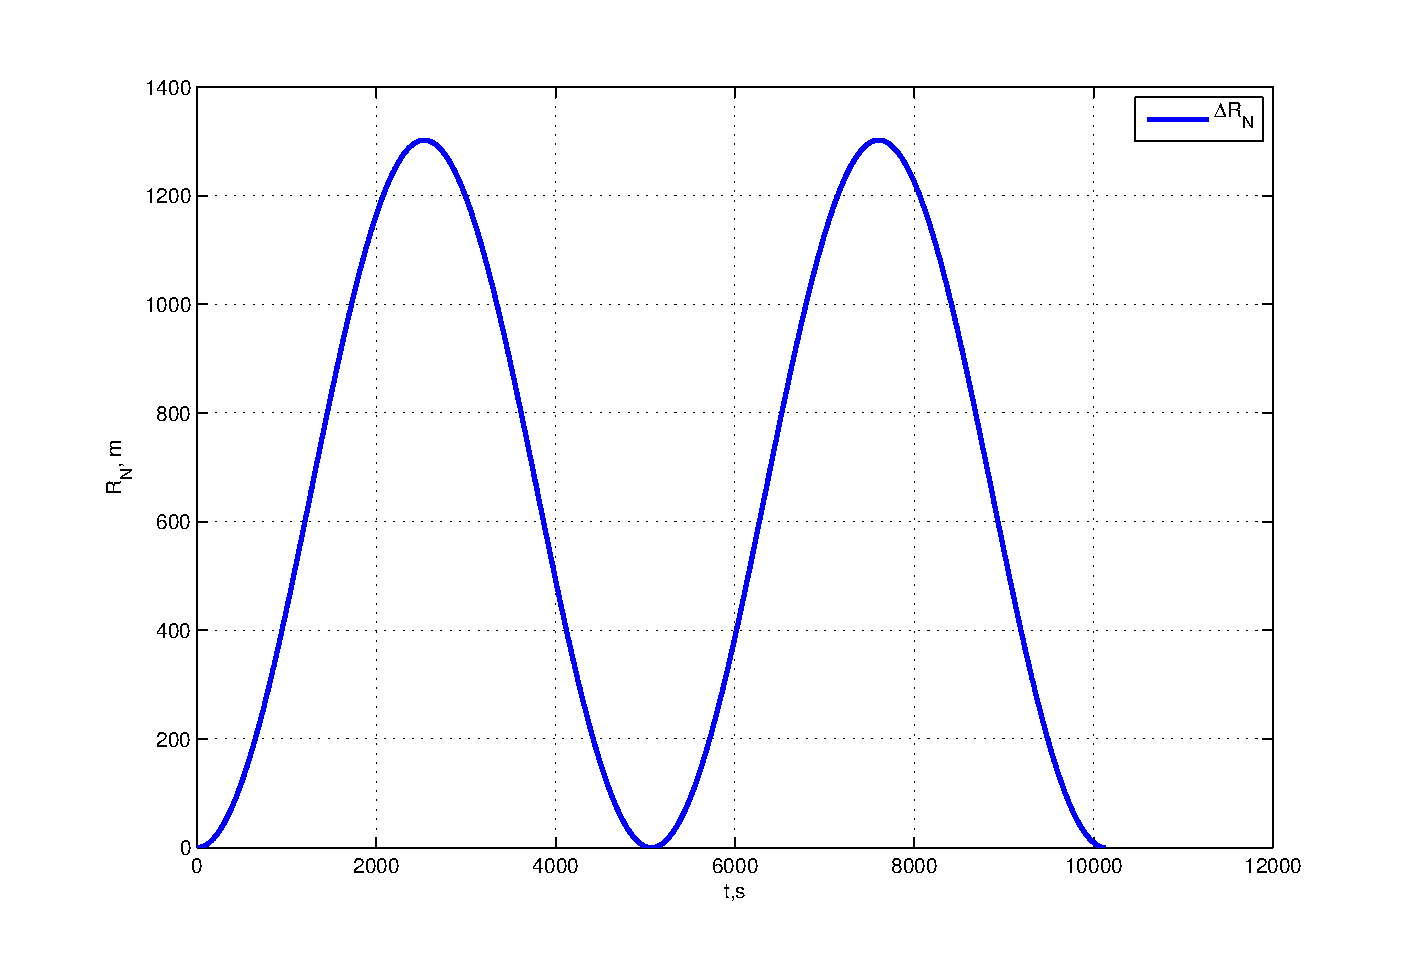
\includegraphics[scale=0.25]{ins_stat_tilt}
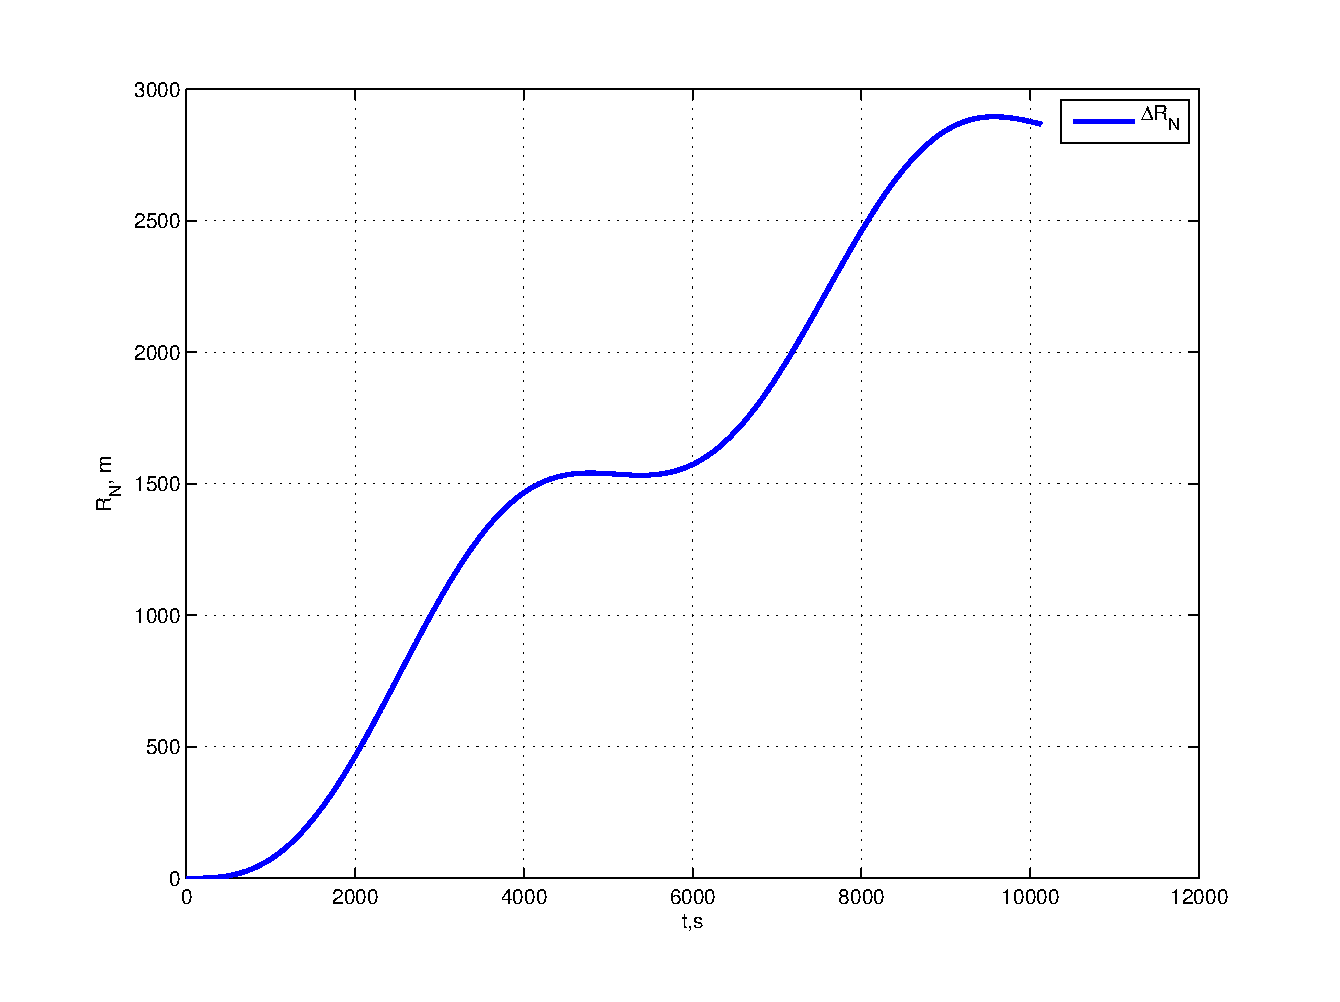
\includegraphics[scale=0.24]{ins_stat_gyro}

\caption{\tiny Еволюція похибки за умови, дрейфу гіроскопа $0.01 deg/h$; Еволюція похибки за умови, похибки координатного тригранника $10^{-3} rad$}
\label{fig:sdins2}
\end{figure}
\end{frame}

%%%%<<<<<<<<<<<<<<<<<<<<<<<<<<<<<<<<<<<<<<<<<<<<<<<<<<<<<<<<<<<<<<<<<<<<<<<<<<<<<<<
\subsection{Сумарна похибка стаціонарно закріпленої БІНС} 
\begin{frame} 
\frametitle{Сумарна похибка стаціонарно закріпленої БІНС}
\begin{figure}[l]
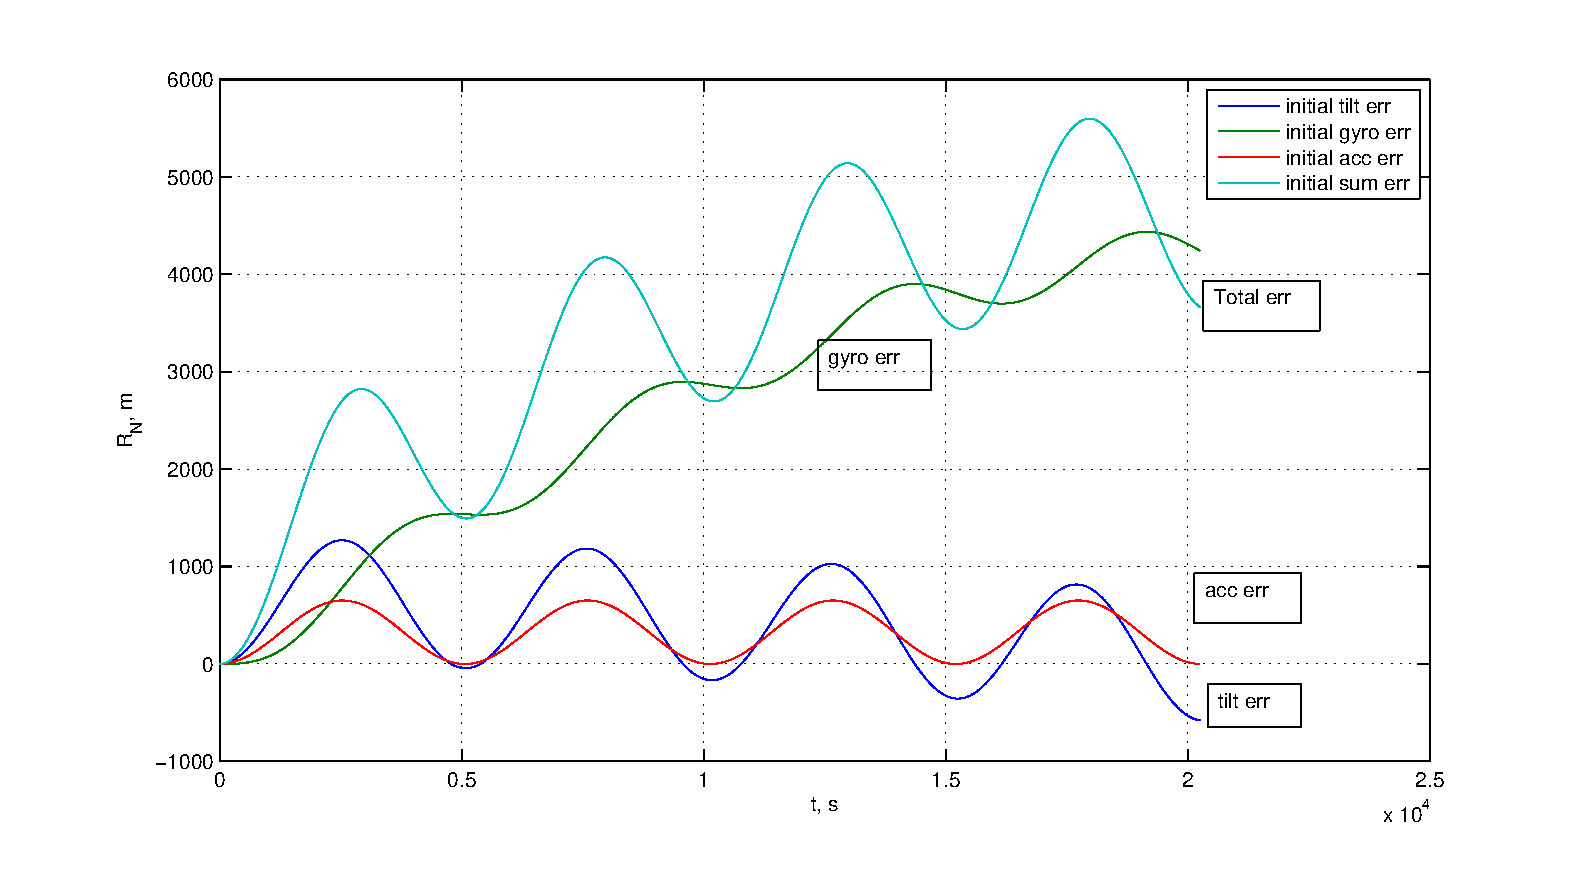
\includegraphics[scale=0.45]{ins_stat_sum}
\caption{\tinyЕволюція сумарної похибки по координаті за умови,
дрейфу гіроскопа   $0.01 deg/h$,похибки координатного тригранника $10^{-3} rad$, та зміщенням акселерометра $10^{-4} m/s^2$}
\label{fig:sdins2}
\end{figure}
\end{frame}

%%%%<<<<<<<<<<<<<<<<<<<<<<<<<<<<<<<<<<<<<<<<<<<<<<<<<<<<<<<<<<<<<<<<<<<<<<<<<<<<<<<
\subsection{Рівняння похибок СНС та БВ} 
\begin{frame} 
\frametitle{Рівняння похибок СНС та БВ}
\tiny
\begin{block}{СНС}
Помилки СНС:\\
$\begin{array}{l} 
{\Delta R_{Es,k} =\Delta R_{Ec,k} +\frac{\sigma_{Rs} }{\cos \varphi_{k} } \eta_{REs,k} +{\color{blue}\frac{\sigma_{\delta Rs} }{\cos \varphi_{k} } \eta_{\delta RE,k}} ;} \\ 
{\Delta R_{Ns,k} =\Delta R_{Nc,k} +\sigma_{Rs} \eta_{RNs,k} +{\color{blue}\sigma_{\delta Rs} \eta_{\delta RN,k}} ;} \\ 
{\Delta H_{s,k} =\Delta H_{c,k} +\sigma_{Hs} \eta_{Hs,k} +{\color{blue}\sigma_{\delta Rs} \eta_{\delta H,k}} }\\ 
{\Delta V_{ls,k} =\Delta V_{lc,k} +\sigma_{Vs} \eta_{V\, ls,k} +{\color{blue}\sigma_{\delta Vs} \eta_{\delta V\, ls,k}}, \text{при } l=E,N,H;} 
\end{array}$\\
Корельовані помилки СНС:\\
$\begin{array}{l} 
{\Delta R_{Ec,k}=W_{R} \Delta R_{Ec,k-1} +q_{R} \frac{\sigma_{Rc} }{\cos \varphi_{k} } \eta_{REc,k} +{\color{blue} \frac{\sigma_{\delta RC} }{\cos \varphi_{k} } \eta_{\delta REc,k}} ;} \\ 
{\Delta R_{Nc,k}=W_{R} \Delta R_{Nc,k-1} +q_{R} \sigma_{Rc} \eta_{RNc,k} +{\color{blue}\sigma_{\delta RC} \eta_{\delta RNc,k}} ;} \\ 
{\Delta H_{c,k}=W_{R}  \Delta H_{c,k-1}  +q_{R} \sigma_{Hc} \eta_{Hc,k} +{\color{blue}\sigma_{\delta Hc} \eta_{\delta Hc,k}} ;} \\ 
{\Delta V_{lc,k} =W_{V} \Delta V_{lc,k-1} +q_{V}\sigma_{Vc} \eta_{V lc,k} +{\color{blue}\sigma_{\delta Vc} \eta_{\delta V lc,k}}, \text{при } l=E,N,H,} 
\end{array} $\\
де:
$\begin{array}{l}
{W_{R} =e^{-(\lambda_{s} V_{\text{Ш}} +\lambda_{st} )\Delta t} ; }
{q_{R} =\left[1-\exp \left(-2\left(\lambda_{s} V_{\text{Ш}} +\lambda_{st} \right)\Delta t\right)\right]^{0,5};}\\
{W_{V} =e^{-\lambda_{V} \Delta t};}
{q_{V} =\left[1-\exp \left(-2 \lambda_{V} \Delta t\right)\right]^{0,5};}

\end{array}$\\
Матриця динаміки корельованих поихибок СНС:
$F_{sns} =\left[\begin{array}{cccccccc} 
{W_{R}} & {.} & {.} & {.} & {.} & {.} \\ 
{.} & {W_{R} } & {.} & {.} & {.} & {.} \\ 
{.} & {.} & {W_{R} } & {.} & {.} & {.} \\ 
{.} & {.} & {.} & {W_{V} } & {.} & {.} \\ 
{.} & {.} & {.} & {.} & {W_{V} } & {.} \\ 
{.} & {.} & {.} & {.} & {.} & {W_{V} } 
\end{array}\right] 
$
\end{block}

\begin{block}{БВ}
Дискретна модель похибок БВ:\\
$\Delta h_{c,k} =\Delta h_{c,k-1} +\sigma_{\xi A} \xi_{k-1}$
\end{block}
\end{frame}
%%%%<<<<<<<<<<<<<<<<<<<<<<<<<<<<<<<<<<<<<<<<<<<<<<<<<<<<<<<<<<<<<<<<<<<<<<<<<<<<<<<
\subsection{Рівняння ІНСН в просторі станів}
\begin{frame}[shrink=5] \frametitle{Система в просторі станів} 

\begin{columns}[t]
\begin{column}{5cm}
\noindent 
Вектор стану системи
\begin{equation*}
\tiny
% \bar{X}= 
\left[ \begin{array}{l}
{{\color{blue}\Delta R_{E}}}\\
{{\color{blue}\Delta R_{N}}}\\
{{\color{blue}\Delta h}}\\
{{\color{blue}\Delta V_{E}}}\\
{{\color{blue}\Delta V_{N}}}\\
{{\color{blue}\Delta V_{h}}}\\
{{\color{blue}\alpha_{E}}}\\
{{\color{blue}\alpha_{N}}}\\
{{\color{blue}\alpha_{h}}}\\
{{\color{blue}\varepsilon_{c1}}}\\
{{\color{blue}\varepsilon_{c2}}}\\
{{\color{blue}\varepsilon_{c3}}}\\
{{\color{blue}\Delta a_{c1}}} \\
{{\color{blue}\Delta a_{c2}}}\\
{{\color{blue}\Delta a_{c3}}}\\
{{\color{red}\Delta h_{\text{БВ}}}}\\
{{\color{violet}\Delta R_{Ec}}}\\
{{\color{violet}\Delta R_{Nc}}}\\
{{\color{violet}\Delta h_{c}}}\\
{{\color{violet}\Delta V_{Ec}}}\\
{{\color{violet}\Delta V_{Nc}}}\\
{{\color{violet}\Delta V_{hc}}}
\end{array} \right]=
\left[\begin{array}{l}
{{\color{blue}\text{Пом. координ. E}}}\\
{{\color{blue}\text{Пом. координ. N}}}\\
{{\color{blue}\text{Пом. по висоті}}}\\
{{\color{blue}\text{Пом. по швидкості E}}}\\
{{\color{blue}\text{Пом. по швидкості N}}}\\
{{\color{blue}\text{Пом. по швидкості H}}}\\
{{\color{blue}\text{Пом. тригранника E}}}\\
{{\color{blue}\text{Пом. тригранника N}}}\\
{{\color{blue}\text{Пом. тригранника H}}}\\
{{\color{blue}\text{Дрейф гіроскопа E}}}\\
{{\color{blue}\text{Дрейф гіроскопа N}}}\\
{{\color{blue}\text{Дрейф гіроскопа H}}}\\
{{\color{blue}\text{Дрейф акселерометра E}}} \\
{{\color{blue}\text{Дрейф акселерометра N}}}\\
{{\color{blue}\text{Дрейф акселерометра H}}}\\
{{\color{red}\text{Пом. баровисотоміра}}}\\
{{\color{violet}\text{Кор. пом. коорд. СНС E}}}\\
{{\color{violet}\text{Кор. пом. коорд. СНС N}}}\\
{{\color{violet}\text{Кор. пом. коорд. СНС H}}}\\
{{\color{violet}\text{Кор. пом. швид. СНС E}}}\\
{{\color{violet}\text{Кор. пом. швид. СНС N}}}\\
{{\color{violet}\text{Кор. пом. швид. СНС H}}}\\
\end{array} \right]  
\end{equation*}

\end{column}
\begin{column}{5cm}
Моедель системи в просторі станів.\\

\tiny

$\bar{X}_{p,k+1} =\Phi_{p,k} \bar{X}_{p,k} +G_{p,k} \bar{\xi }_{k}$ \\
Матриця динаміки системи\\
$ F_{p,k} =\left[\begin{array}{ccc} 
{F_{k} } & {.} & {.} \\
{.} & {F_{bv}} & {.} \\
{.} & {.} & {F_{sns}} \\
\end{array}\right];$
Коваріаційна матриця шумів\\
$Q_{p,k} =\left[\begin{array}{ccc} 
{Q_{k} } & {.} & {.} \\ 
{.} & {\sigma_{\text{БВ}} \sqrt{\Delta t}} & {.} \\ 
{.} & {.} & {G_{s,k} } \end{array}\right];$
Вимірювання\\
$\bar{Y}_{k} = 
\left[\begin{array}{l}
{\tilde{h}_{k} -\tilde{h}_{\text{БВ},k},}\\
{\tilde{R}_{E,K} -\tilde{R}_{ES,k},}\\
{\tilde{R}_{N,K} -\tilde{R}_{NS,k},}\\
{\tilde{h}_{k} -\tilde{h}_{s,k},}\\
{\tilde{V}_{E,k} -\tilde{V}_{ES,k},}\\
{\tilde{V}_{N,k} -\tilde{V}_{NS,k},}\\
{\tilde{V}_{h,k} -\tilde{V}_{hS,k},}\\
{\tilde{h}_{\text{БВ}} -\tilde{h}_{s,k}}
\end{array} \right] $
\end{column}
\end{columns}
\end{frame}


%%%%<<<<<<<<<<<<<<<<<<<<<<<<<<<<<<<<<<<<<<<<<<<<<<<<<<<<<<<<<<<<<<<<<<<<<<<<<<<<<<<
\subsection{Навігаційний фільтр Калмана} 
\begin{frame}%[plain]
\frametitle{Навігаційний фільтр Калмана}
\begin{figure}[l]
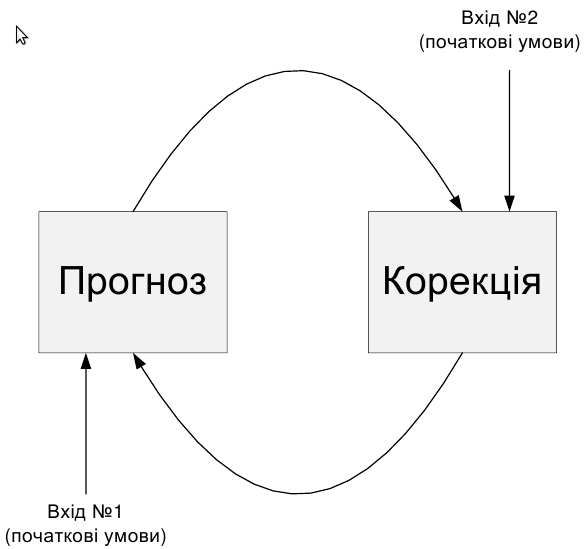
\includegraphics[scale=0.15]{kalman_diag}
% \caption{\tinyЕволюція сумарної }
\end{figure}
\begin{block}{Фільтр Калмана}
\small
Прогноз: \\
$\begin{array}{l} 
{\hat{\bar{X}}_{p,k}(-) =\Phi_{p,k-1} \hat{\bar{X}}_{p,k-1}(+) ,} \\ 
{P_{k}(-) =\Phi_{p,k-1} P_{k-1}(+) \Phi ^{T}_{p,k-1} +G_{p,k-1} G_{p,k-1}^{T} ;} \end{array} $ \\
Корекція:\\
$\begin{array}{l} 
{\hat{\bar{X}}_{p,k}(+)=\hat{\bar{X}}_{p,k}(-) + K_{k} (\bar{Y}_{k} -H\hat{\bar{X}}_{p,k} )} \\ 
{P_{k}(+)={\color{blue}(E-K_{k} H)P_{k}(-) \left(E-K_{k} H\right)^{T}} +{\color{red} K_{k} Q_{p,k} Q_{p,k} ^{T} K_{k}^{T}} } 
\end{array} $ \\
Коефіцієнт Калмана:\\
$K_{k} =P_{k}(-) H^{T} (HP_{k}(-) H^{T} +Q_{p,k} Q_{p,k} ^{T} )^{-1} $
\end{block}
\end{frame}
%%%%<<<<<<<<<<<<<<<<<<<<<<<<<<<<<<<<<<<<<<<<<<<<<<<<<<<<<<<<<<<<<<<<<<<<<<<<<<<<<<<
\subsection{Виправлення координат} 
\begin{frame}%[plain]
\frametitle{Виправлення координат}
Виправлення координат:\\
$\begin{array}{l} 
{h(+)_{i} =h(-)_{i} -\Delta \hat{h}_{i} ;} \\ 
{\varphi_{i}(+) =\varphi (-)_{i} -\frac{\Delta \hat{R}_{Ni} }{R_{\text{З}} } ;} \\ 
{\lambda_{i}(+) =\lambda (-)_{i} -\frac{\Delta \hat{R}_{Ei} }{R_{\text{З}} } ;} \\ 
\end{array} $\\
Виправлення швидкостей:\\
$\begin{array}{l}
{V(+)_{E}=V(-)_{E} -\Delta \hat{V}_{E}; } \\
{V(+)_{N}=V(-)_{N} -\Delta \hat{V}_{N}; } \\
{V(+)_{h}=V(-)_{h} -\Delta \hat{V}_{h}. } 
\end{array} $\\
Виправлення орієнтації географічної СК:\\
$\hat{B}(+)_{i} =\Delta B_{i} \hat{B}(-)_{i}$

$\Delta B_{i} =\left[\begin{array}{ccc} 
{1} & {-\hat{\alpha }_{h,i} } & {\hat{\alpha }_{N,i} }\\ 
{\hat{\alpha }_{h,i} } & {1} & {-\hat{\alpha }_{E,i} }\\ 
{-\hat{\alpha }_{N,i} } & {\hat{\alpha }_{E,i} } & {1} \end{array}\right]$.                                              
%  
% $\stackrel{\frown}{\alpha }_{E,i} $, 
% $\stackrel{\frown}{\alpha }_{N,i} $, 
% $\stackrel{\frown}{\alpha }_{h,i} $

% \begin{block}{Фільтр Калмана}
% \end{block}
\end{frame}

%%%%<<<<<<<<<<<<<<<<<<<<<<<<<<<<<<<<<<<<<<<<<<<<<<<<<<<<<<<<<<<<<<<<<<<<<<<<<<<<<<<
\section{Моделювання ІСНС} 
\subsection{Програмне забезпечення} 
\begin{frame}%[plain]
\frametitle{Інтерфейс програми}
\begin{figure}
\centering
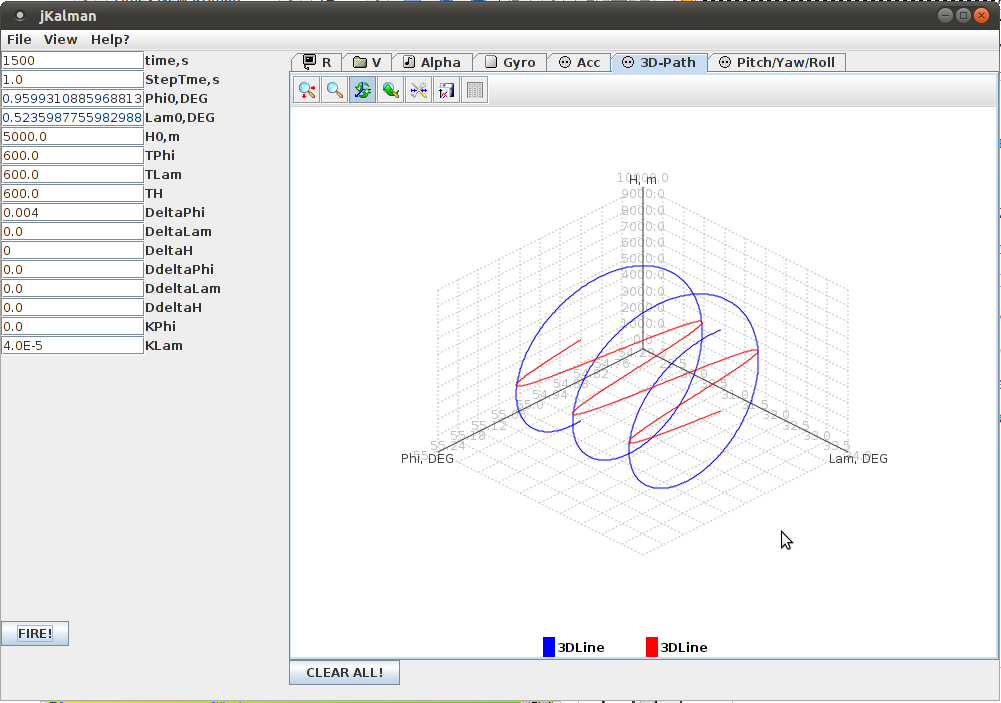
\includegraphics[scale=0.25]{3d_soft}
% \caption{\tiny Траєкторія руху ЛА та його кути орієнтації }
\end{figure}
\end{frame}

%%%%<<<<<<<<<<<<<<<<<<<<<<<<<<<<<<<<<<<<<<<<<<<<<<<<<<<<<<<<<<<<<<<<<<<<<<<<<<<<<<<
\subsection{Похибка оцінки по координаті} 
\begin{frame}%[plain]
\frametitle{Похибка оцінки по координаті}
\noindent
\begin{figure}
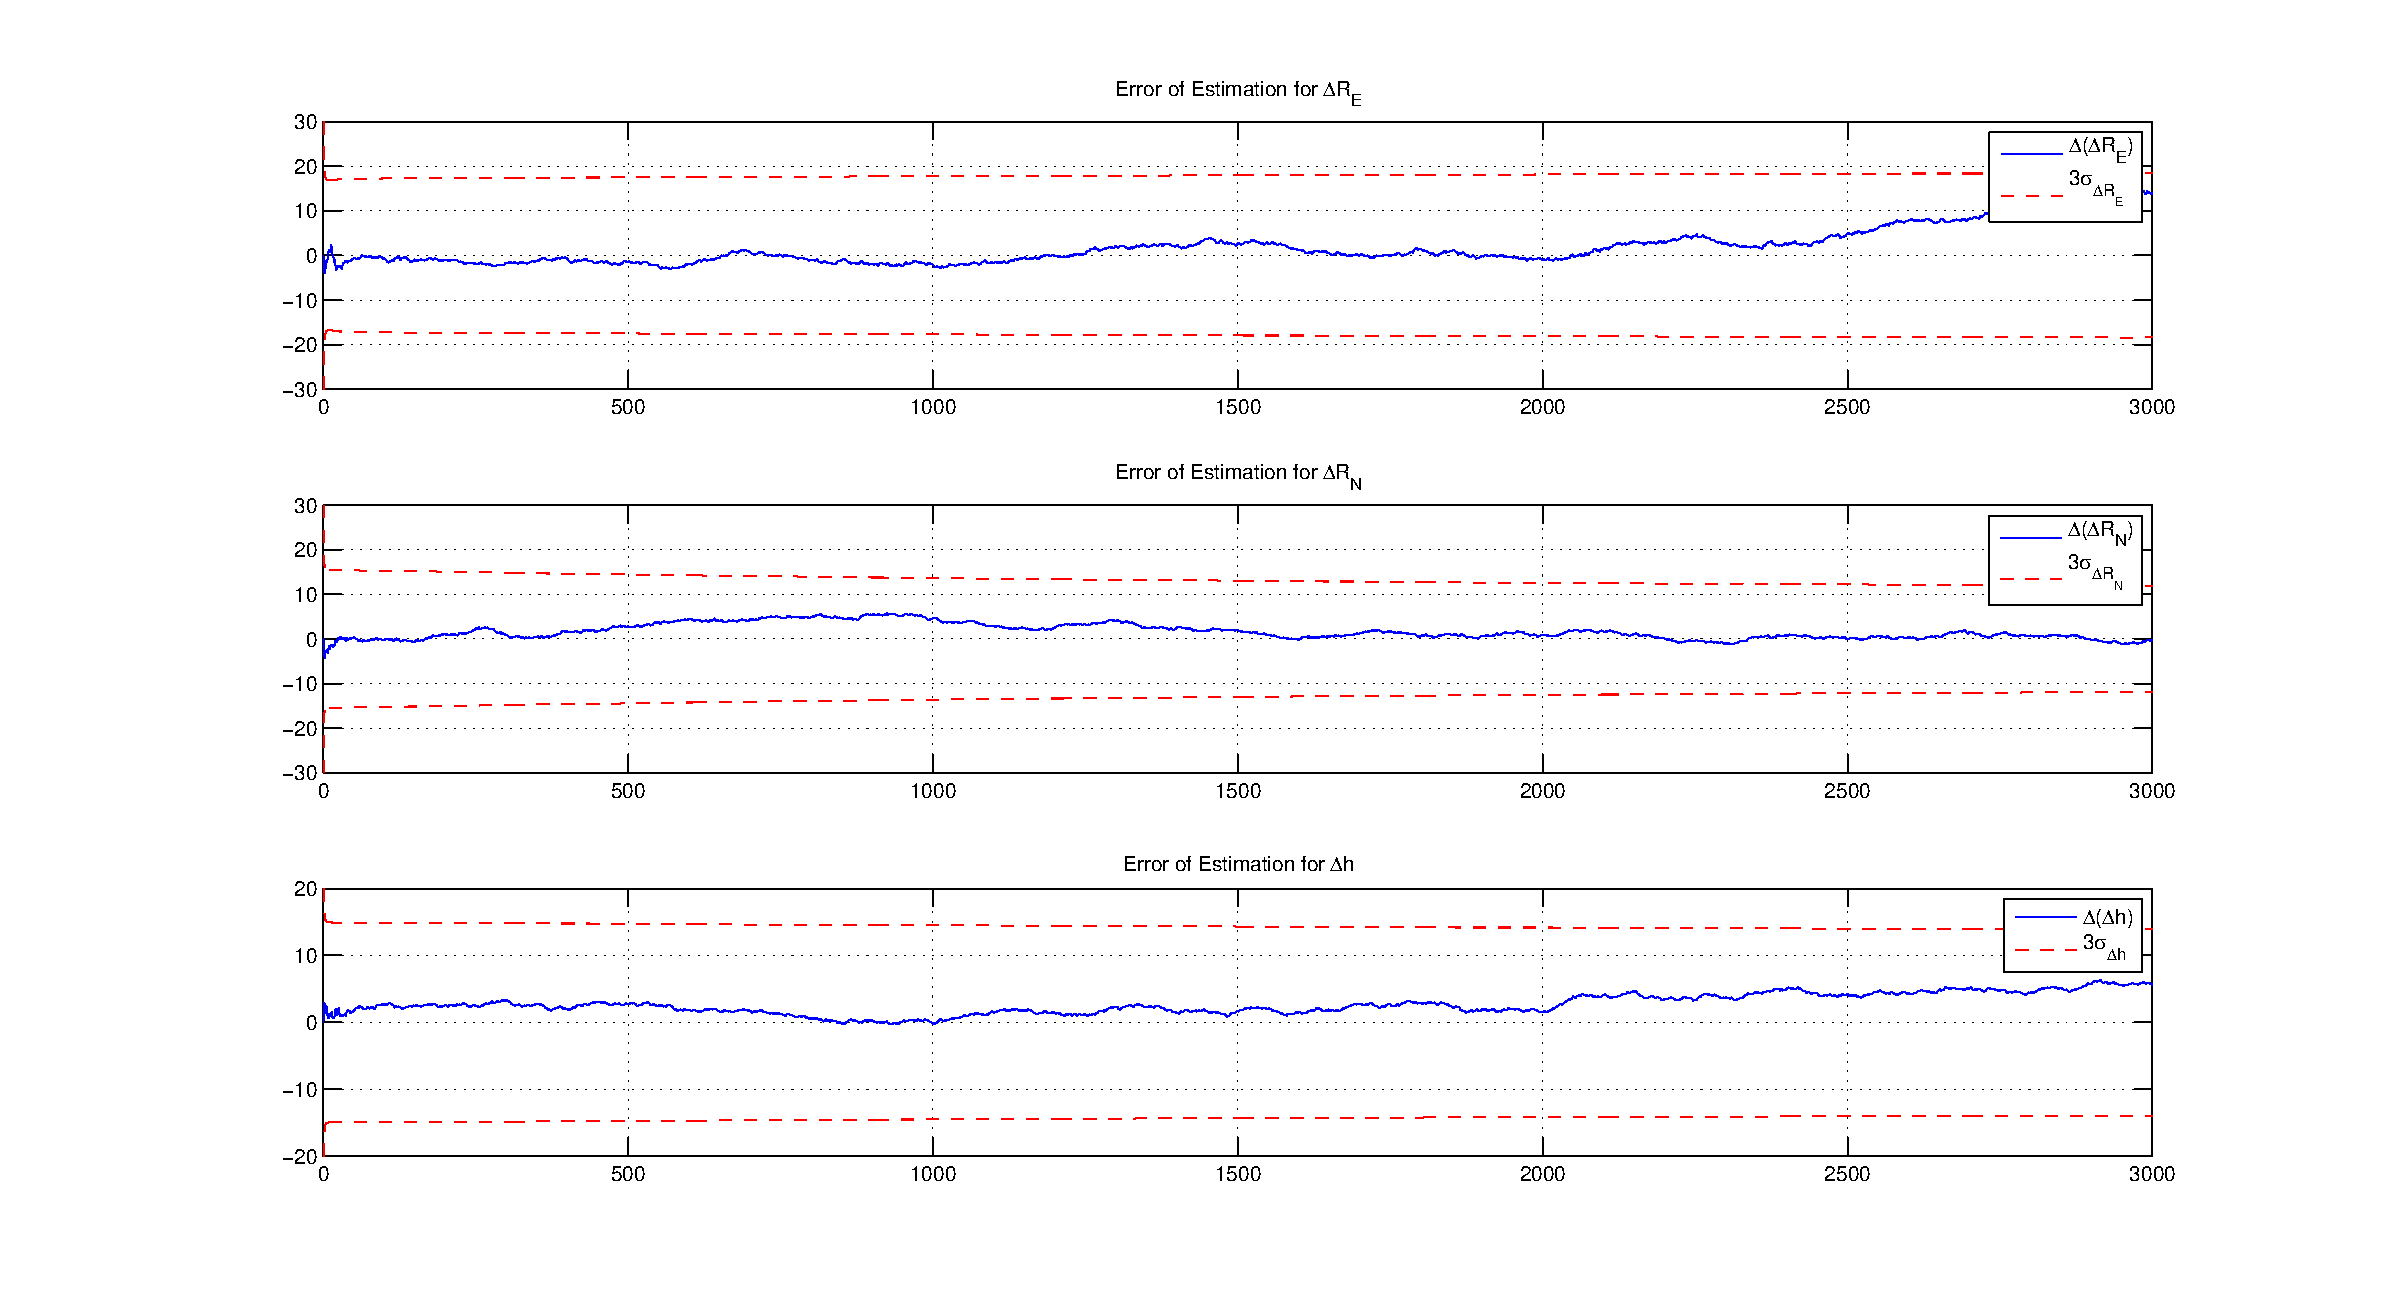
\includegraphics[scale=0.3]{ErrEstCovR}
% \caption{\tiny Траєкторія руху ЛА та його кути орієнтації }
\end{figure}
\end{frame}

%%%%<<<<<<<<<<<<<<<<<<<<<<<<<<<<<<<<<<<<<<<<<<<<<<<<<<<<<<<<<<<<<<<<<<<<<<<<<<<<<<<
\subsection{Похибка оцінки по швидкості} 
\begin{frame}%[plain]
\frametitle{Похибка оцінки по швидкості}
\noindent
\begin{figure}
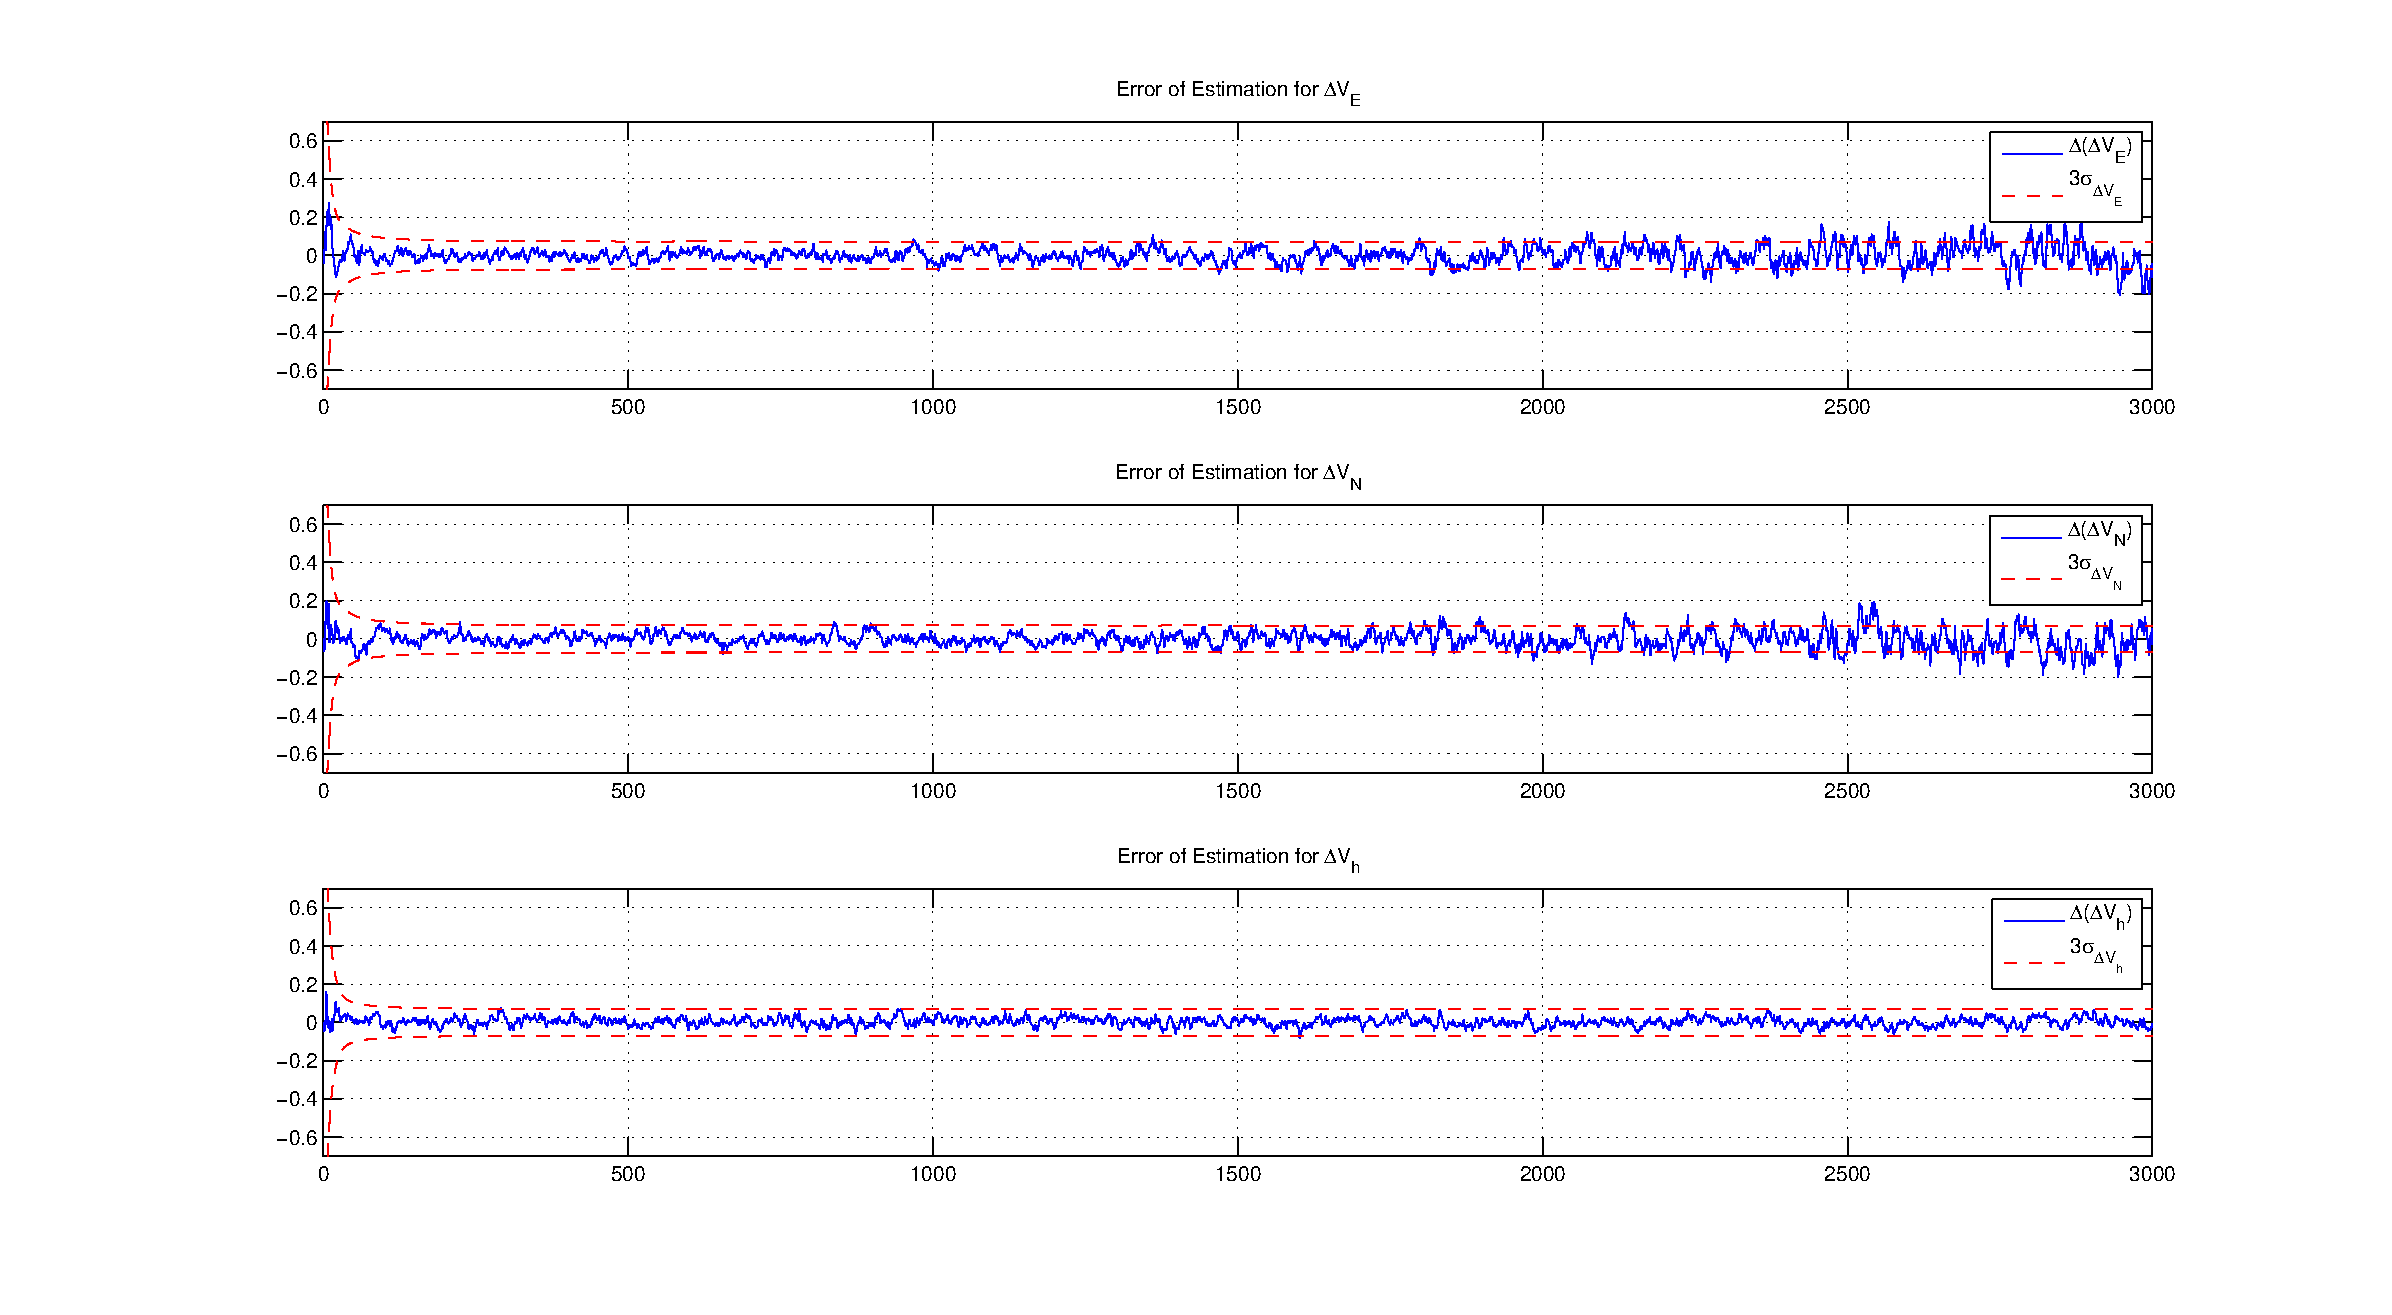
\includegraphics[scale=0.3]{ErrEstCovV}
% \caption{\tiny Траєкторія руху ЛА та його кути орієнтації }
\end{figure}
\end{frame}

%%%%<<<<<<<<<<<<<<<<<<<<<<<<<<<<<<<<<<<<<<<<<<<<<<<<<<<<<<<<<<<<<<<<<<<<<<<<<<<<<<<
\subsection{Похибка оцінки по орієнтації} 
\begin{frame}%[plain]
\frametitle{Похибка оцінки по орієнтації}
\noindent
\begin{figure}
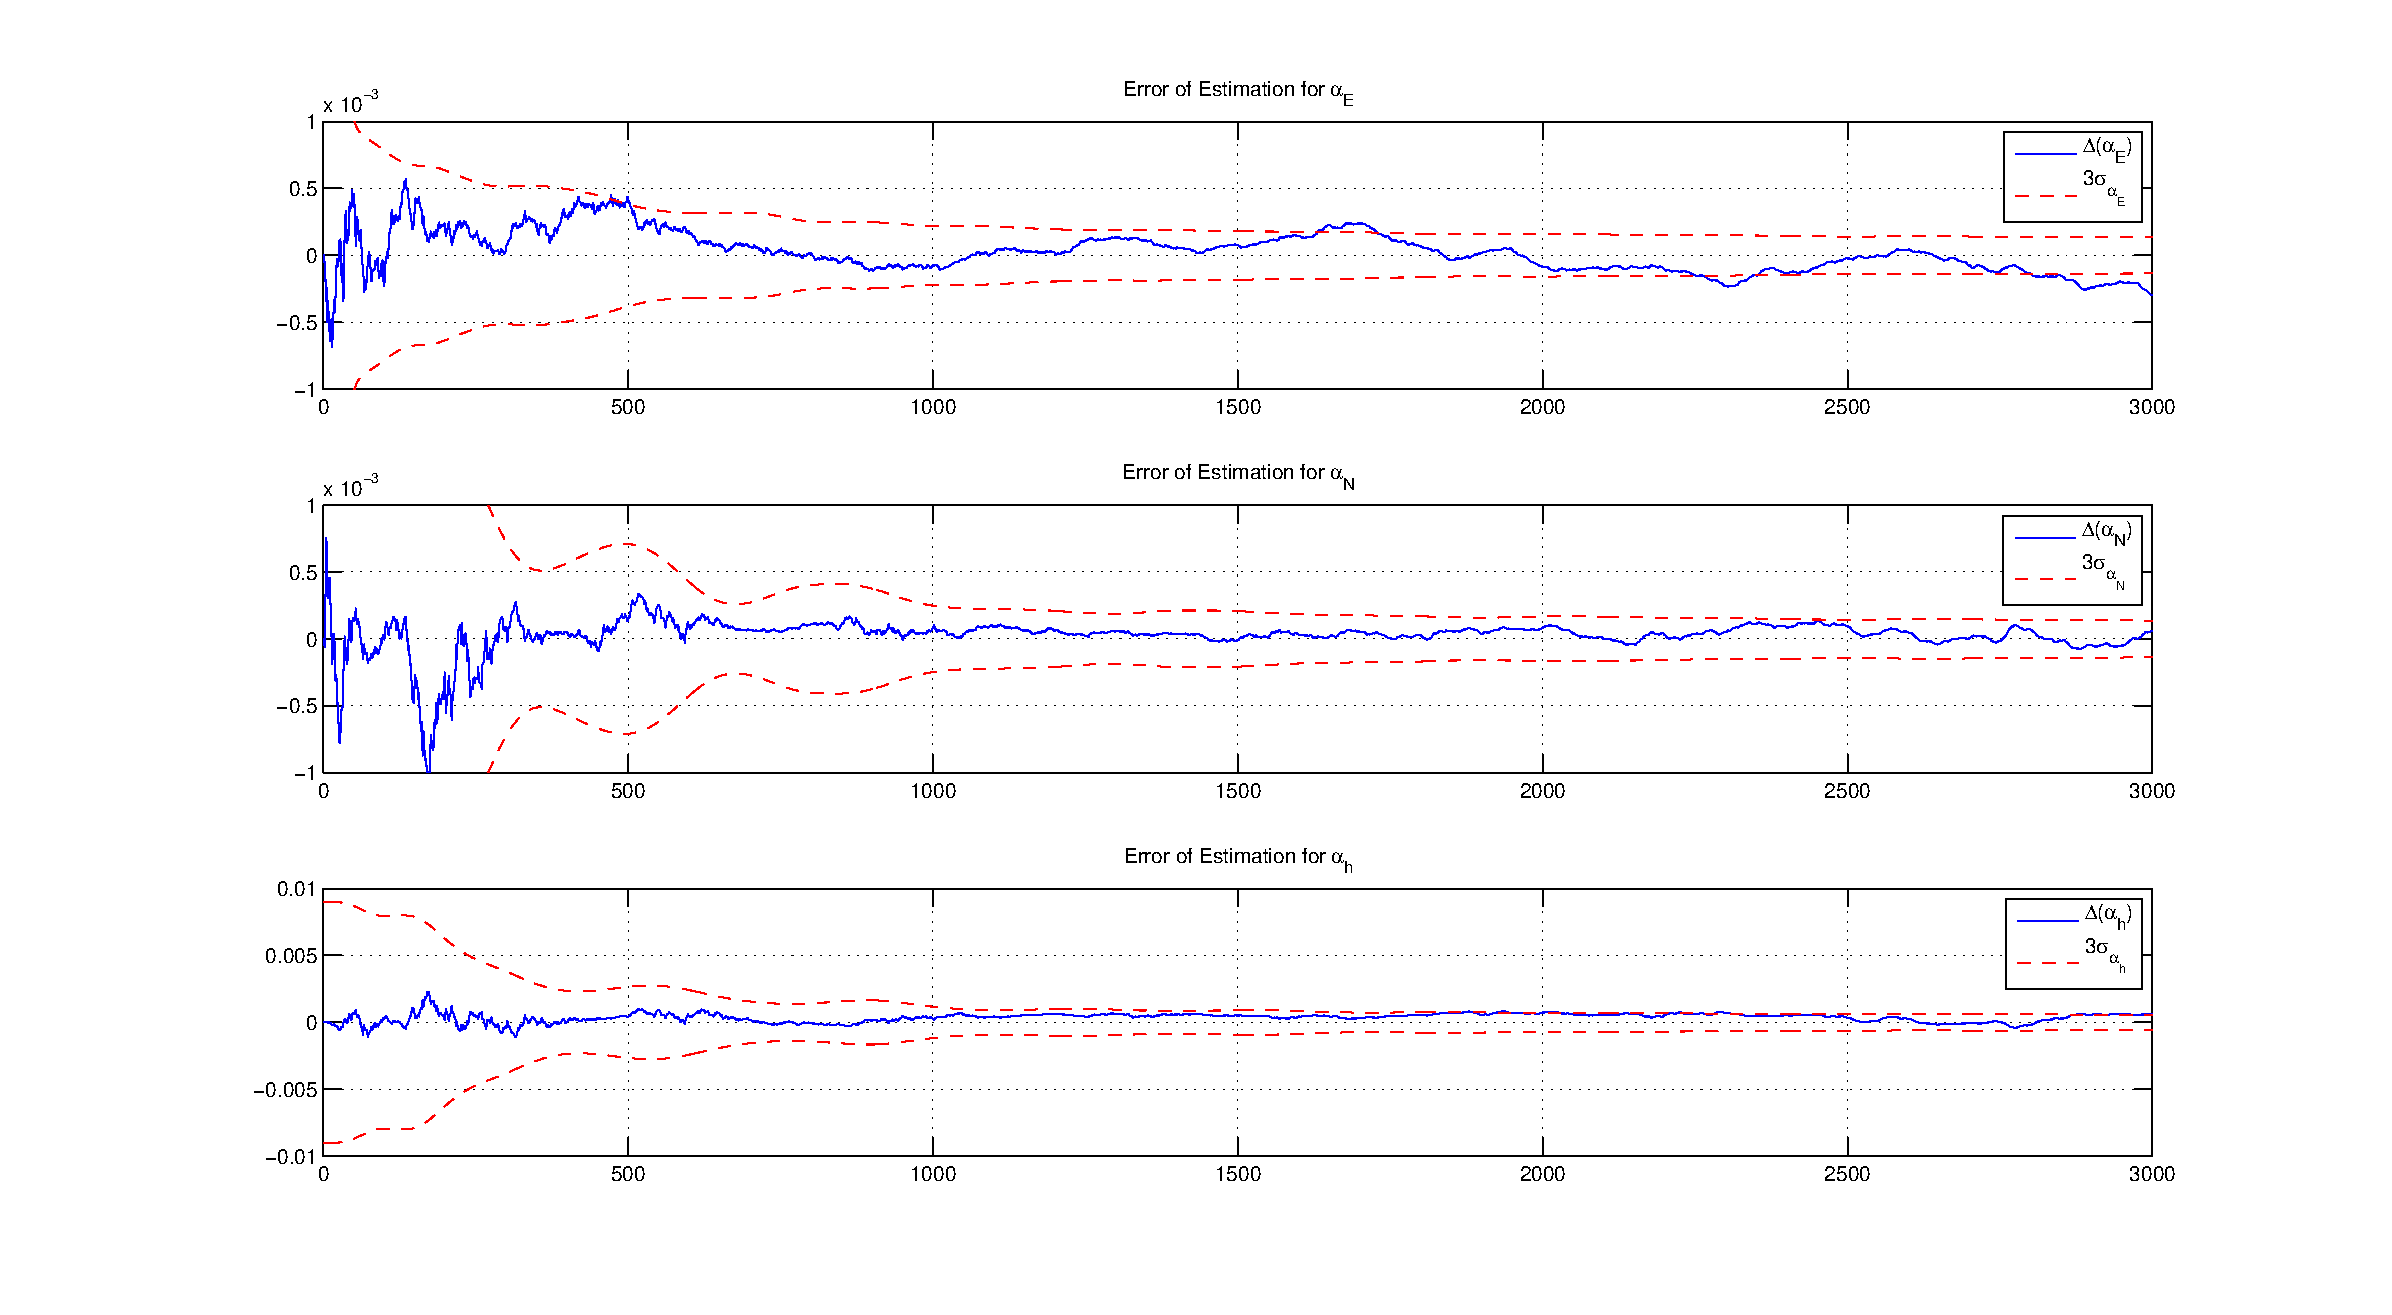
\includegraphics[scale=0.3]{ErrEstCovAlph}
% \caption{\tiny Траєкторія руху ЛА та його кути орієнтації }
\end{figure}
\end{frame}

%%%%<<<<<<<<<<<<<<<<<<<<<<<<<<<<<<<<<<<<<<<<<<<<<<<<<<<<<<<<<<<<<<<<<<<<<<<<<<<<<<<
\subsection{Похибка оцінки дрейфів гіроскопів} 
\begin{frame}%[plain]
\frametitle{Похибка оцінки дрейфів гіроскопів}
\noindent
\begin{figure}
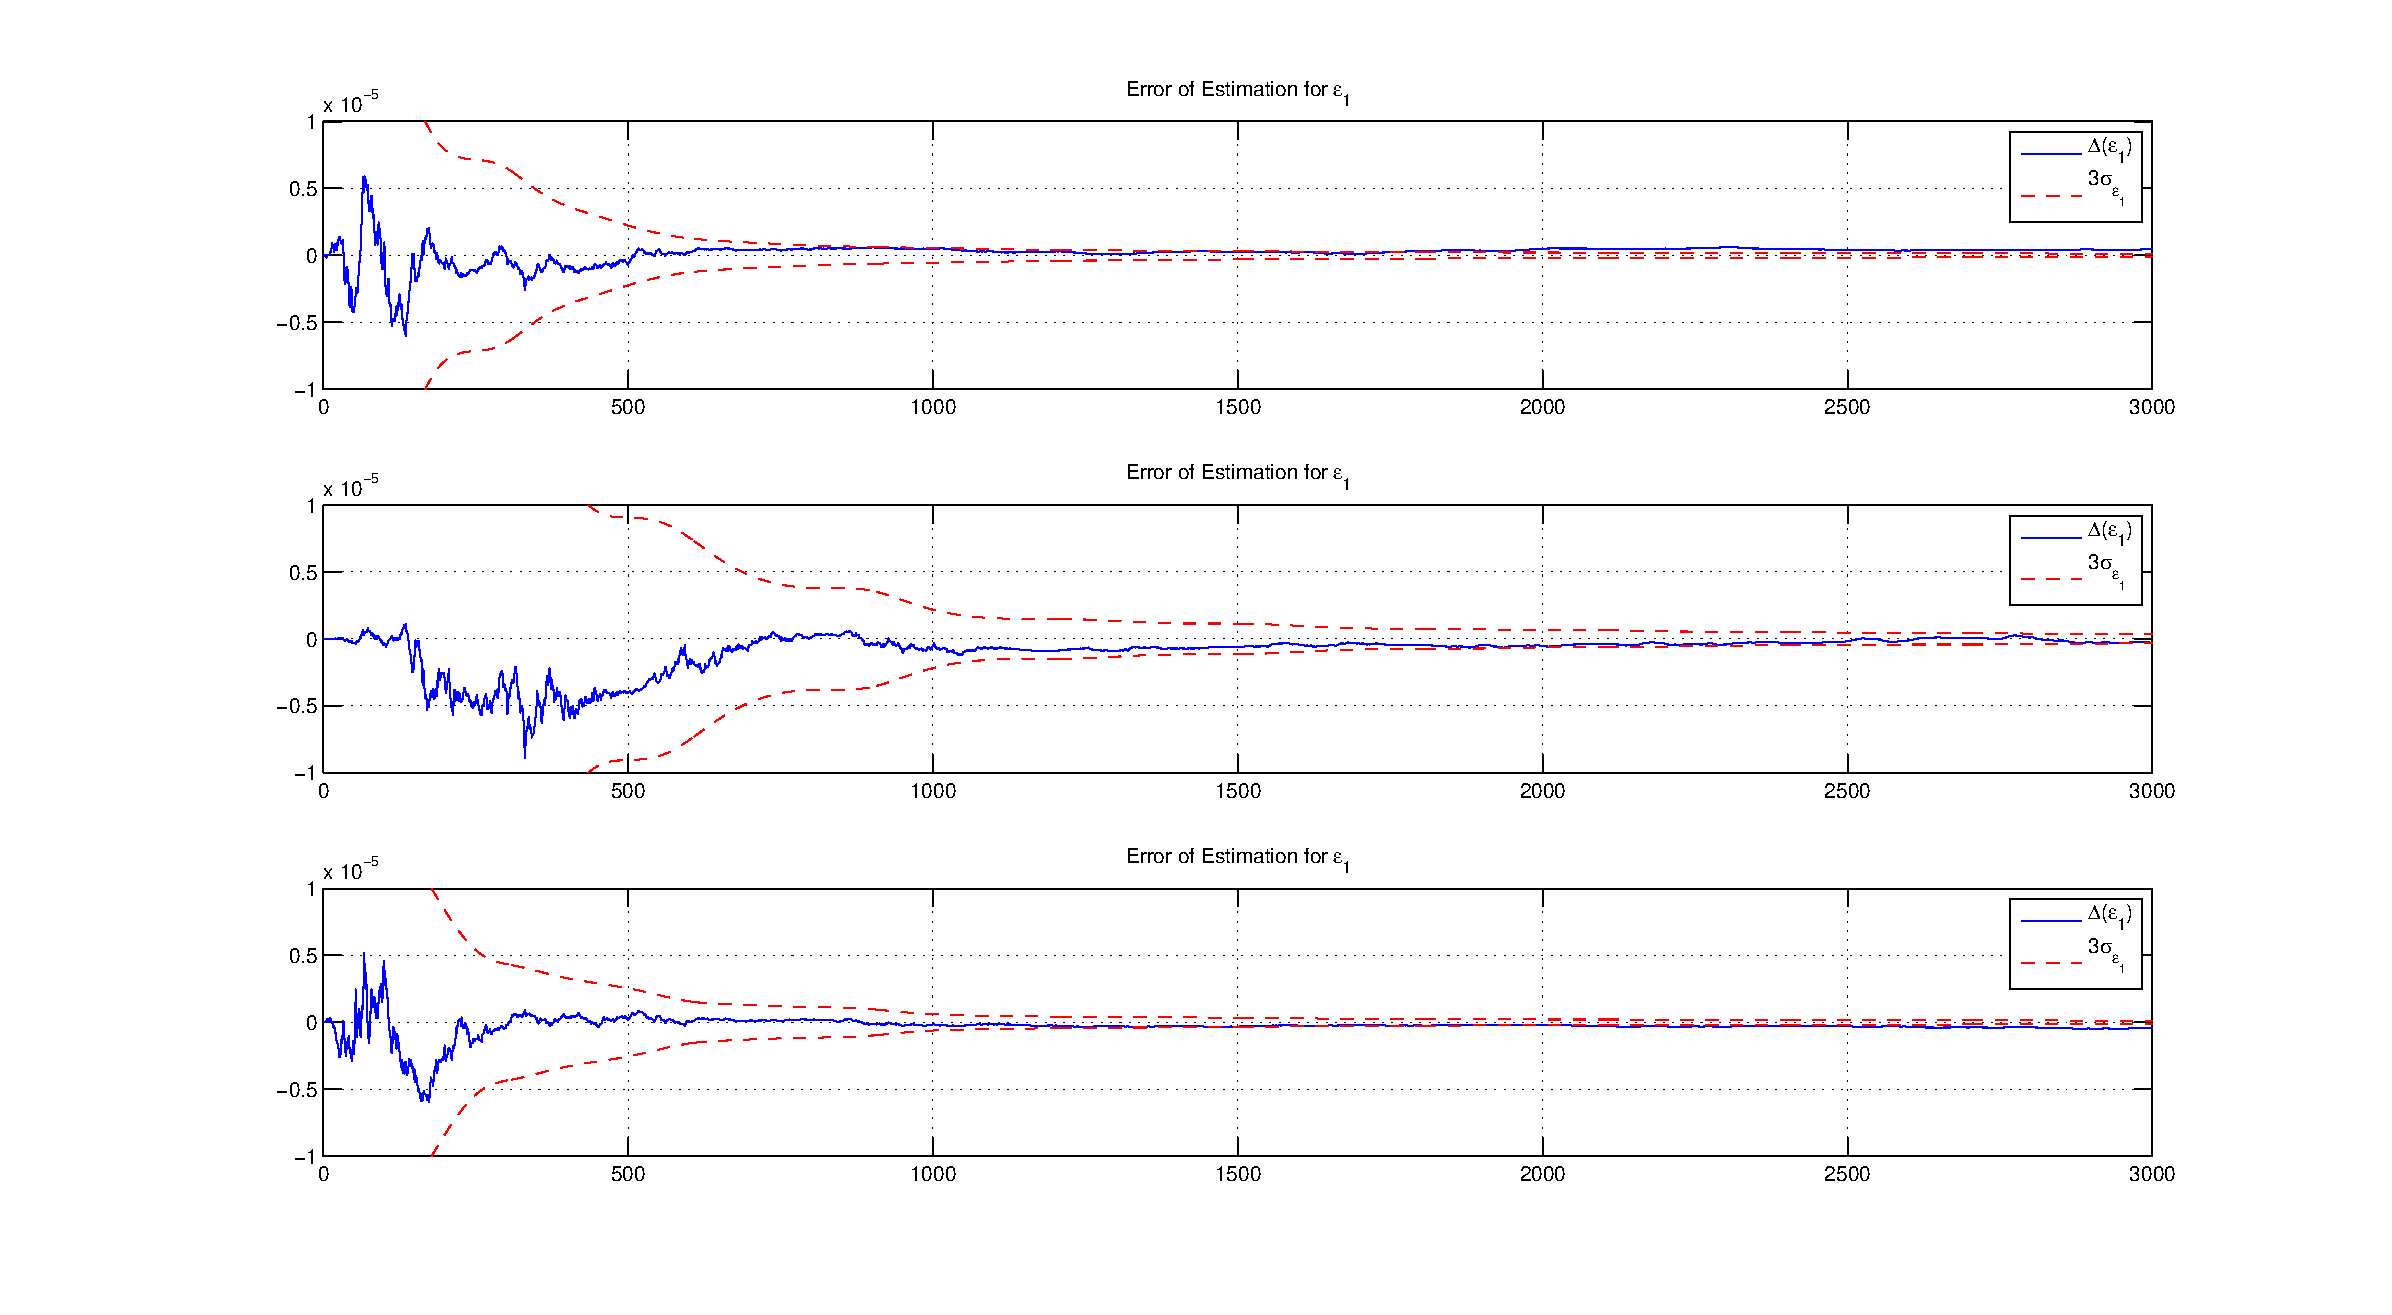
\includegraphics[scale=0.3]{ErrEstCovGyro}
% \caption{\tiny Траєкторія руху ЛА та його кути орієнтації }
\end{figure}
\end{frame}

%%%%<<<<<<<<<<<<<<<<<<<<<<<<<<<<<<<<<<<<<<<<<<<<<<<<<<<<<<<<<<<<<<<<<<<<<<<<<<<<<<<
\subsection{Похибка оцінки зміщення акселерометрів} 
\begin{frame}%[plain]
\frametitle{Похибка оцінки зміщення акселерометрів}
\begin{figure}
\centering
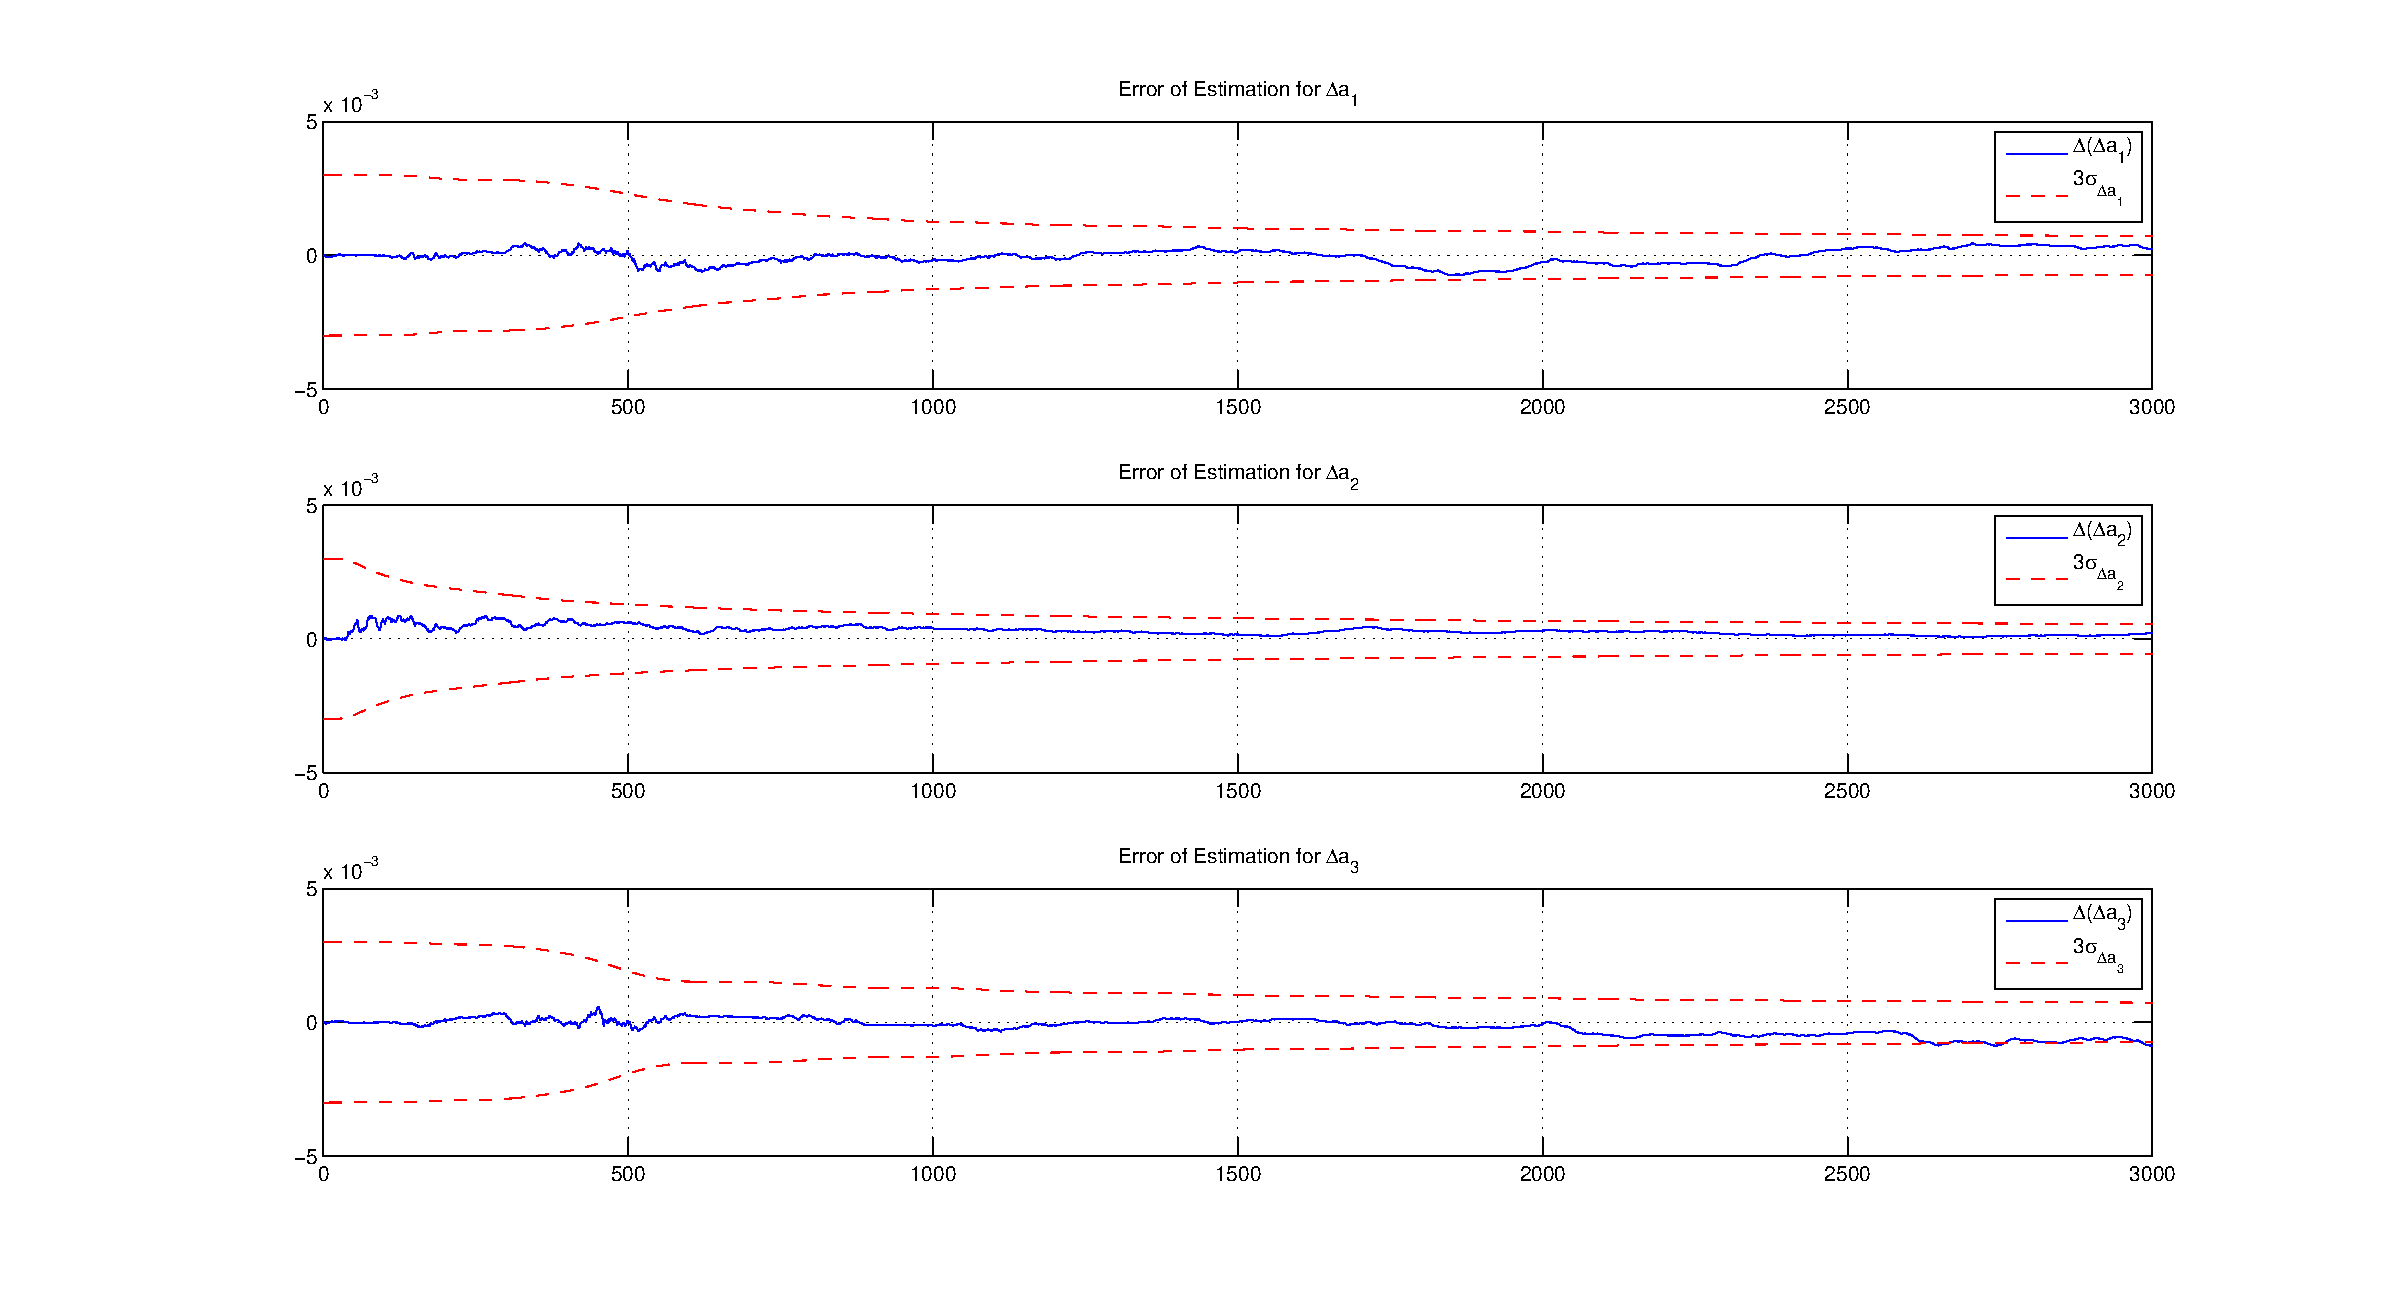
\includegraphics[scale=0.3]{ErrEstCovAcc}
% \caption{\tiny Траєкторія руху ЛА та його кути орієнтації }
\end{figure}
\end{frame}
%%%%<<<<<<<<<<<<<<<<<<<<<<<<<<<<<<<<<<<<<<<<<<<<<<<<<<<<<<<<<<<<<<<<<<<<<<<<<<<<<<<
\subsection{Похибка оцінки курсу, крена, тангажа} 
\begin{frame}%[plain]
\frametitle{Похибка оцінки курсу, крена, тангажа}
\begin{figure}
\centering
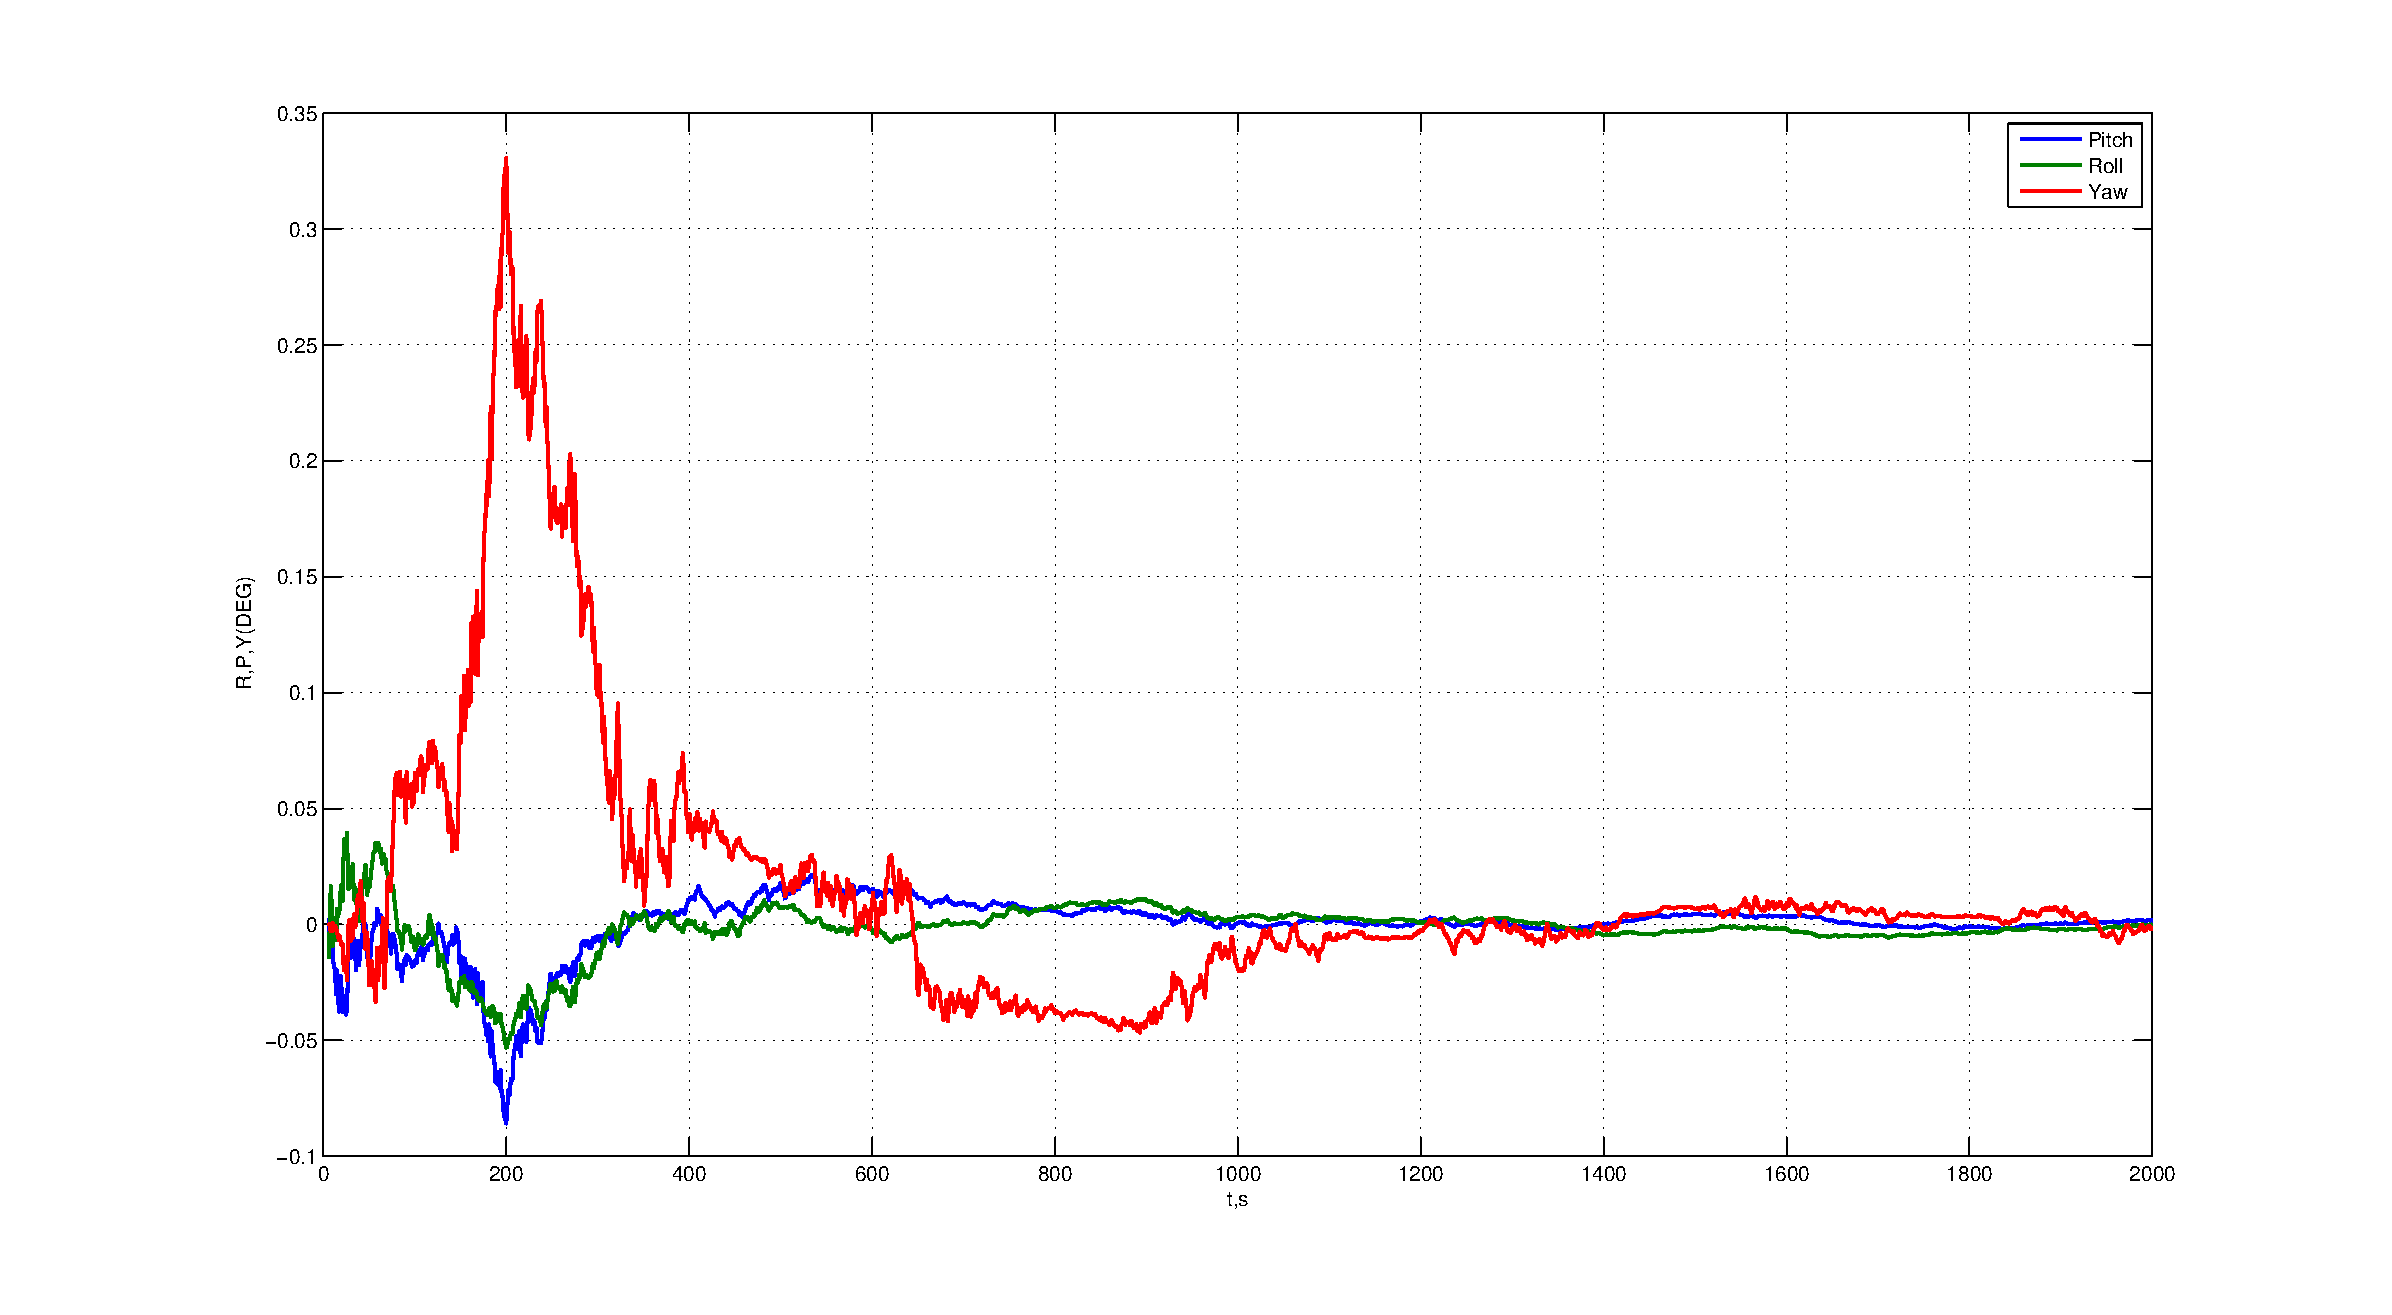
\includegraphics[scale=0.25]{ErrEstAngle3}
% \caption{\tiny Траєкторія руху ЛА та його кути орієнтації }
\end{figure}
\end{frame}
% %%%%<<<<<<<<<<<<<<<<<<<<<<<<<<<<<<<<<<<<<<<<<<<<<<<<<<<<<<<<<<<<<<<<<<<<<<<<<<<<<<<
% \subsection{Сходимість коваріацій параметрів} 
% \begin{frame}%[plain]
% \frametitle{Сходимість коваріацій параметрів}
% \begin{figure}
% \centering
% 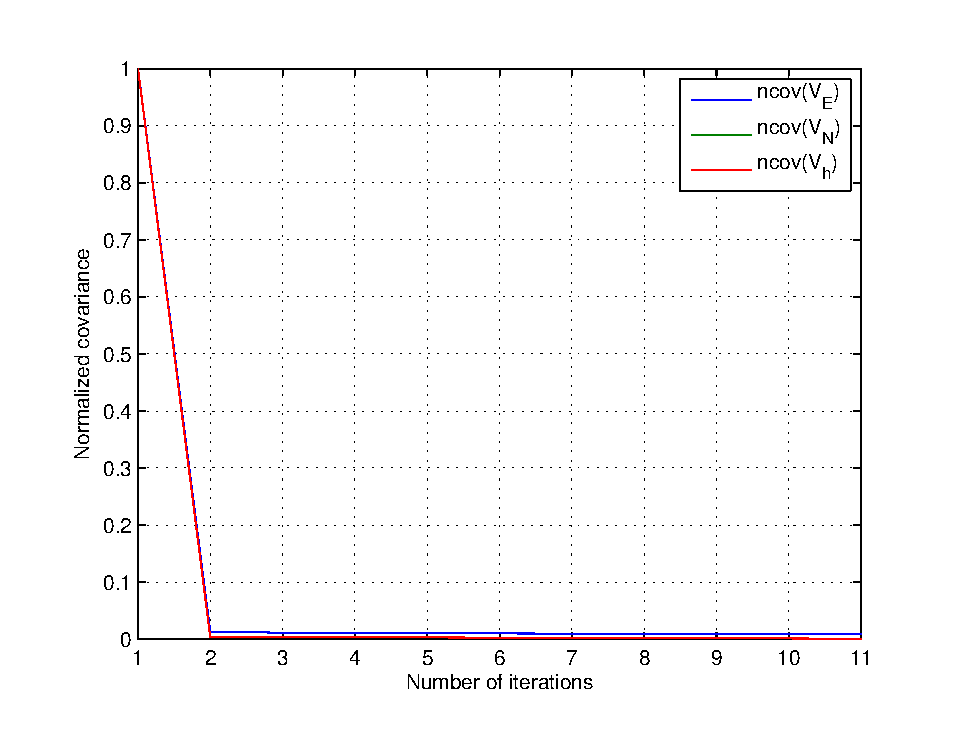
\includegraphics[ width=60mm, height=30.0mm]{cov_v}
% 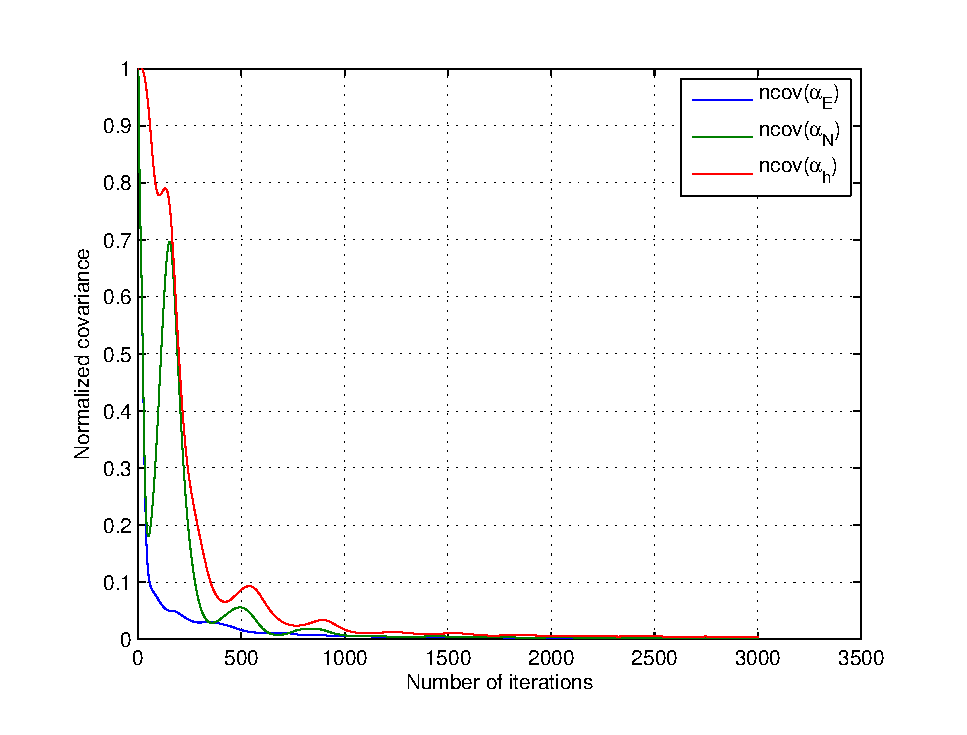
\includegraphics[ width=60mm, height=30.0mm]{cov_alpha}\\
% 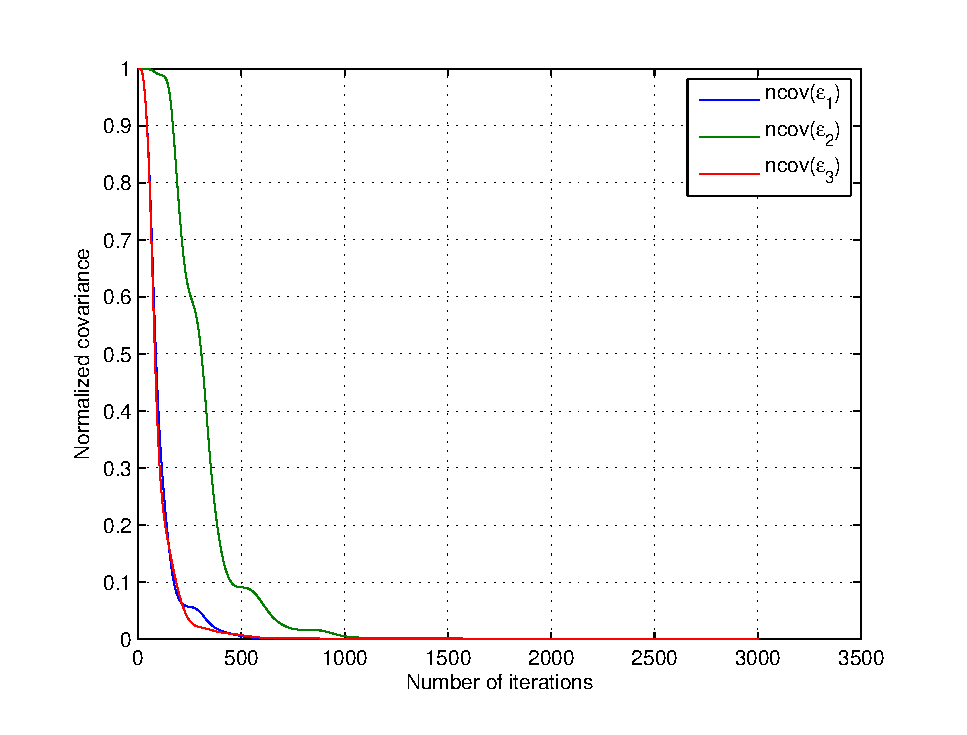
\includegraphics[ width=60mm, height=30.0mm]{cov_eps}
% 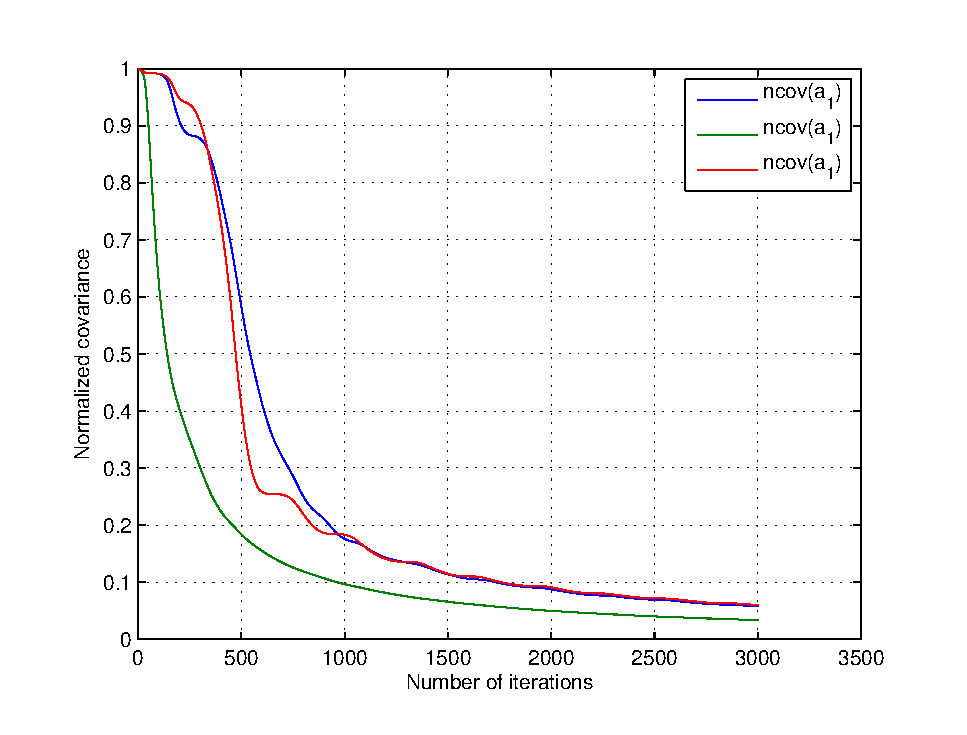
\includegraphics[ width=60mm, height=30.0mm]{cov_a}
% \caption{\tiny Сходимість нормалізованих коваріацій швидкостей, орієнтації, дрейфу гіроскопів та зміщення акселерометрів}
% \end{figure}
% \end{frame}

%%%%<<<<<<<<<<<<<<<<<<<<<<<<<<<<<<<<<<<<<<<<<<<<<<<<<<<<<<<<<<<<<<<<<<<<<<<<<<<<<<<
\subsection{Помилка при відмові СНС} 
\begin{frame}%[plain]
\frametitle{Радіомовчання з 400-600с}
\begin{figure}
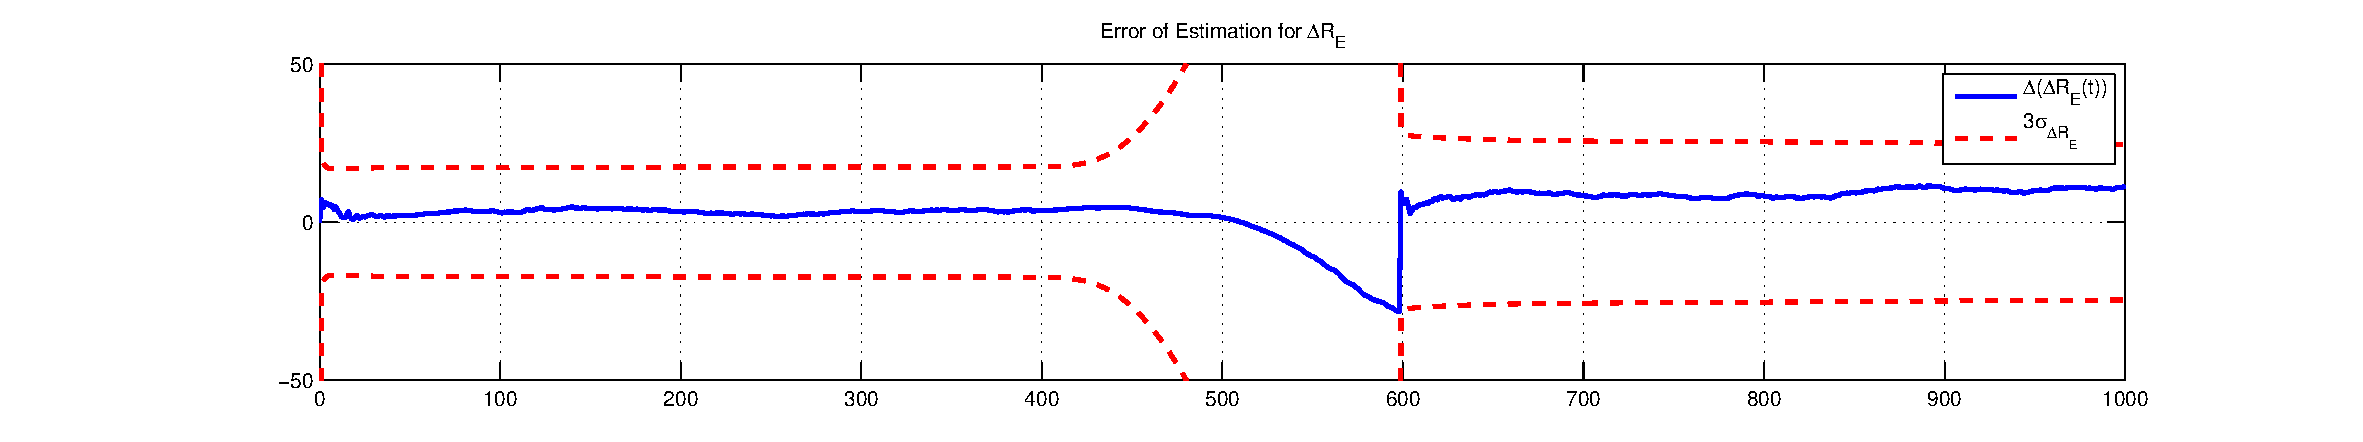
\includegraphics[scale=0.3]{snsless_400_600_R}\\
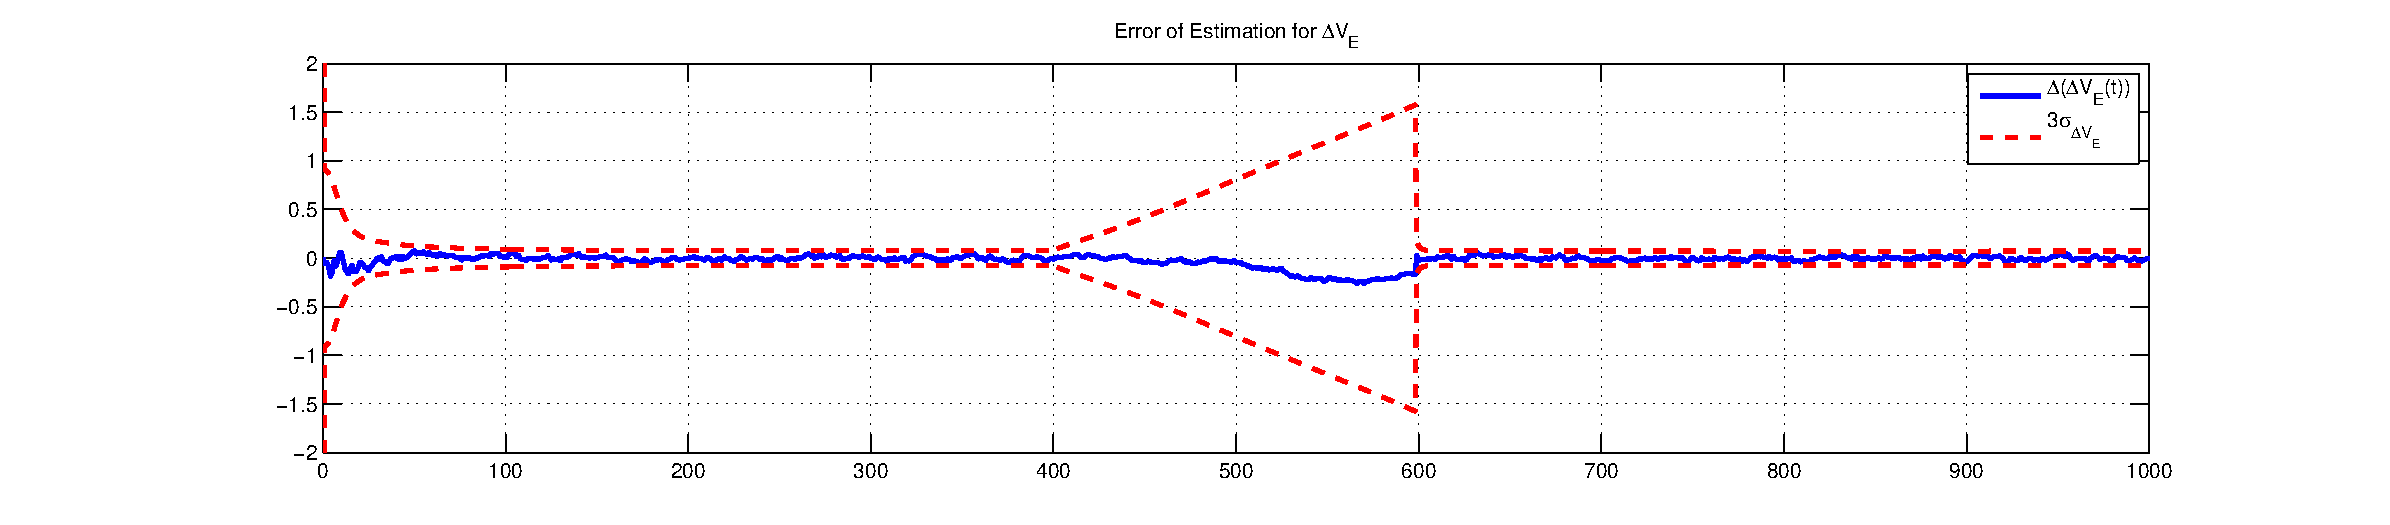
\includegraphics[scale=0.3]{snsless_400_600_V}\\
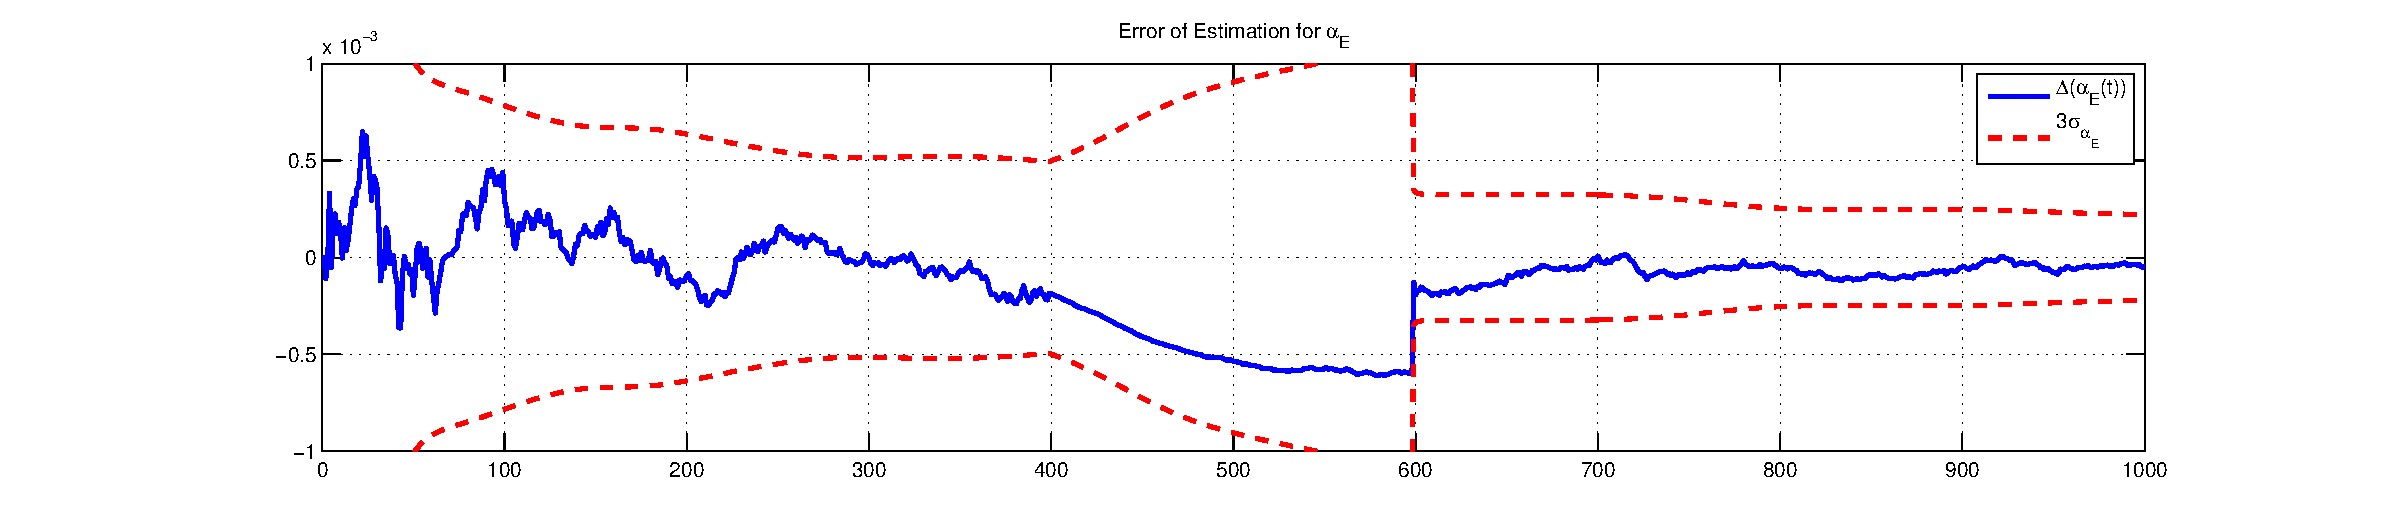
\includegraphics[scale=0.3]{snsless_400_600_alpha}\\
\end{figure}
\end{frame}

% %%%%<<<<<<<<<<<<<<<<<<<<<<<<<<<<<<<<<<<<<<<<<<<<<<<<<<<<<<<<<<<<<<<<<<<<<<<<<<<<<<<
% \subsection{Траєкторія руху ЛА за БІНС і ФК при відмові СНС} 
% \begin{frame}%[plain]
% \frametitle{Траєкторія руху за БІНС і ФК}
% \noindent
% \begin{figure}[l]
% % \noindent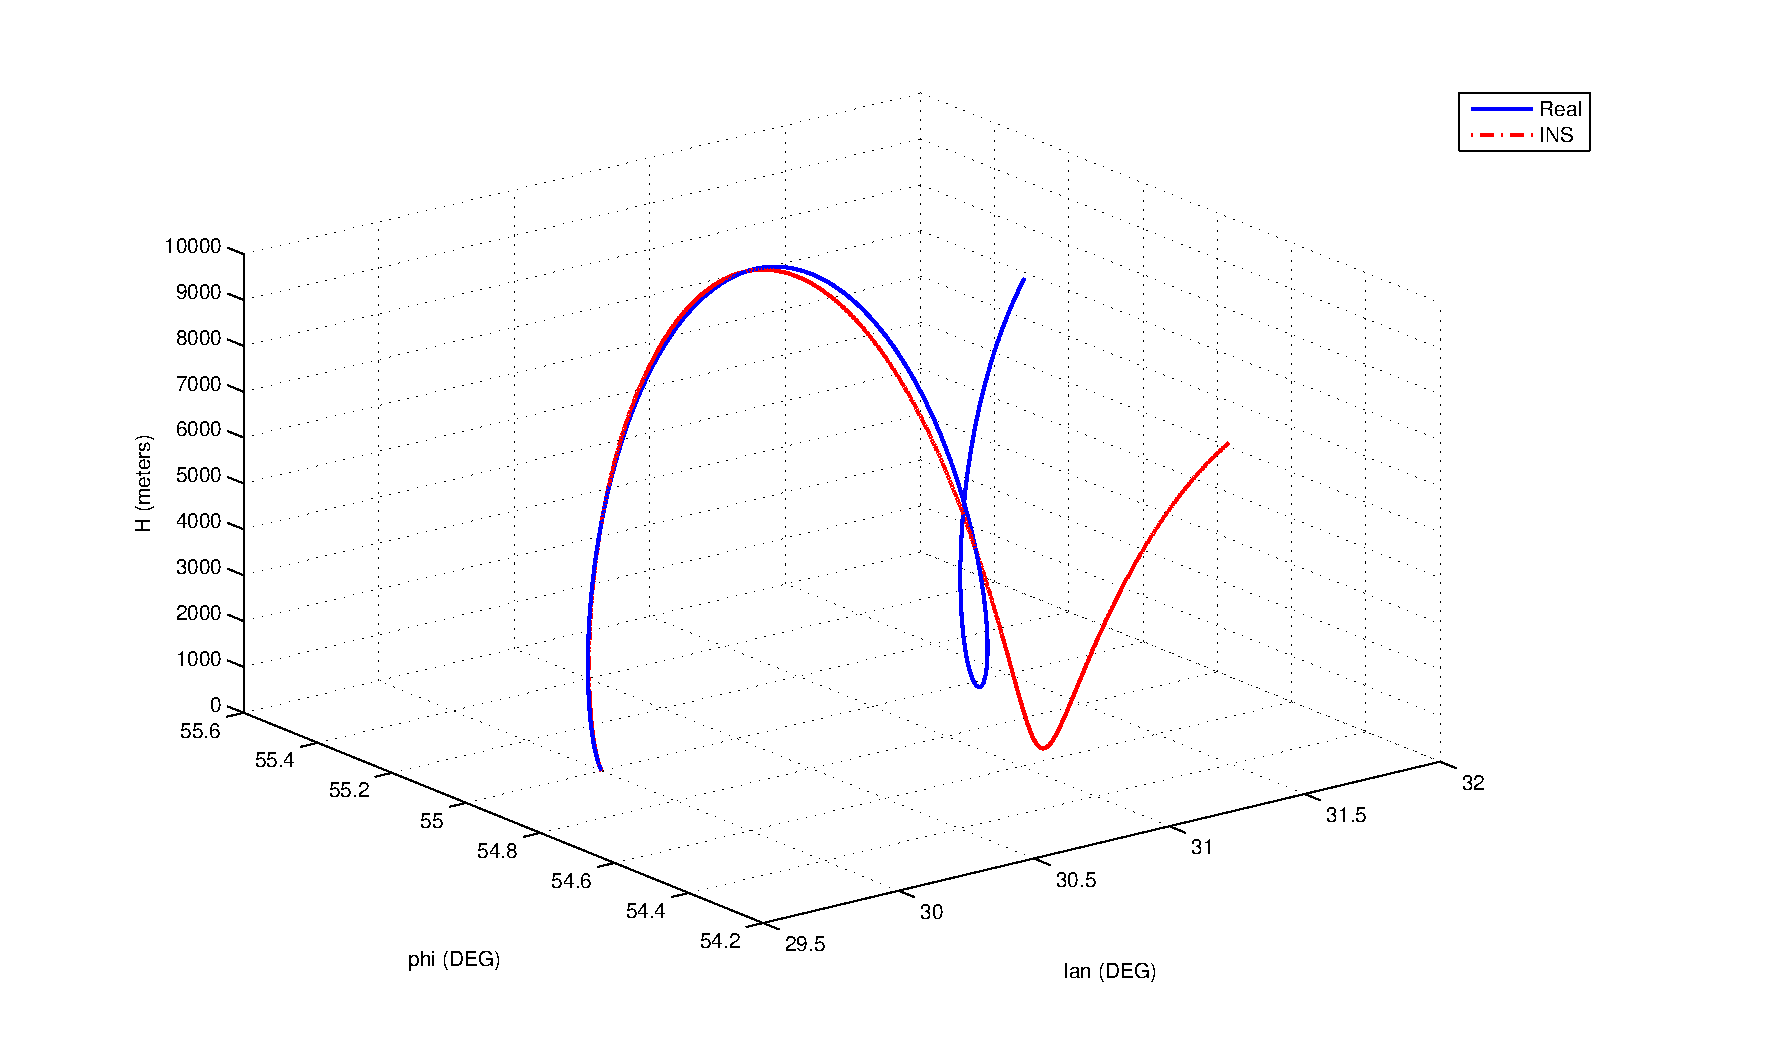
\includegraphics[scale=0.2]{only_ins}
% 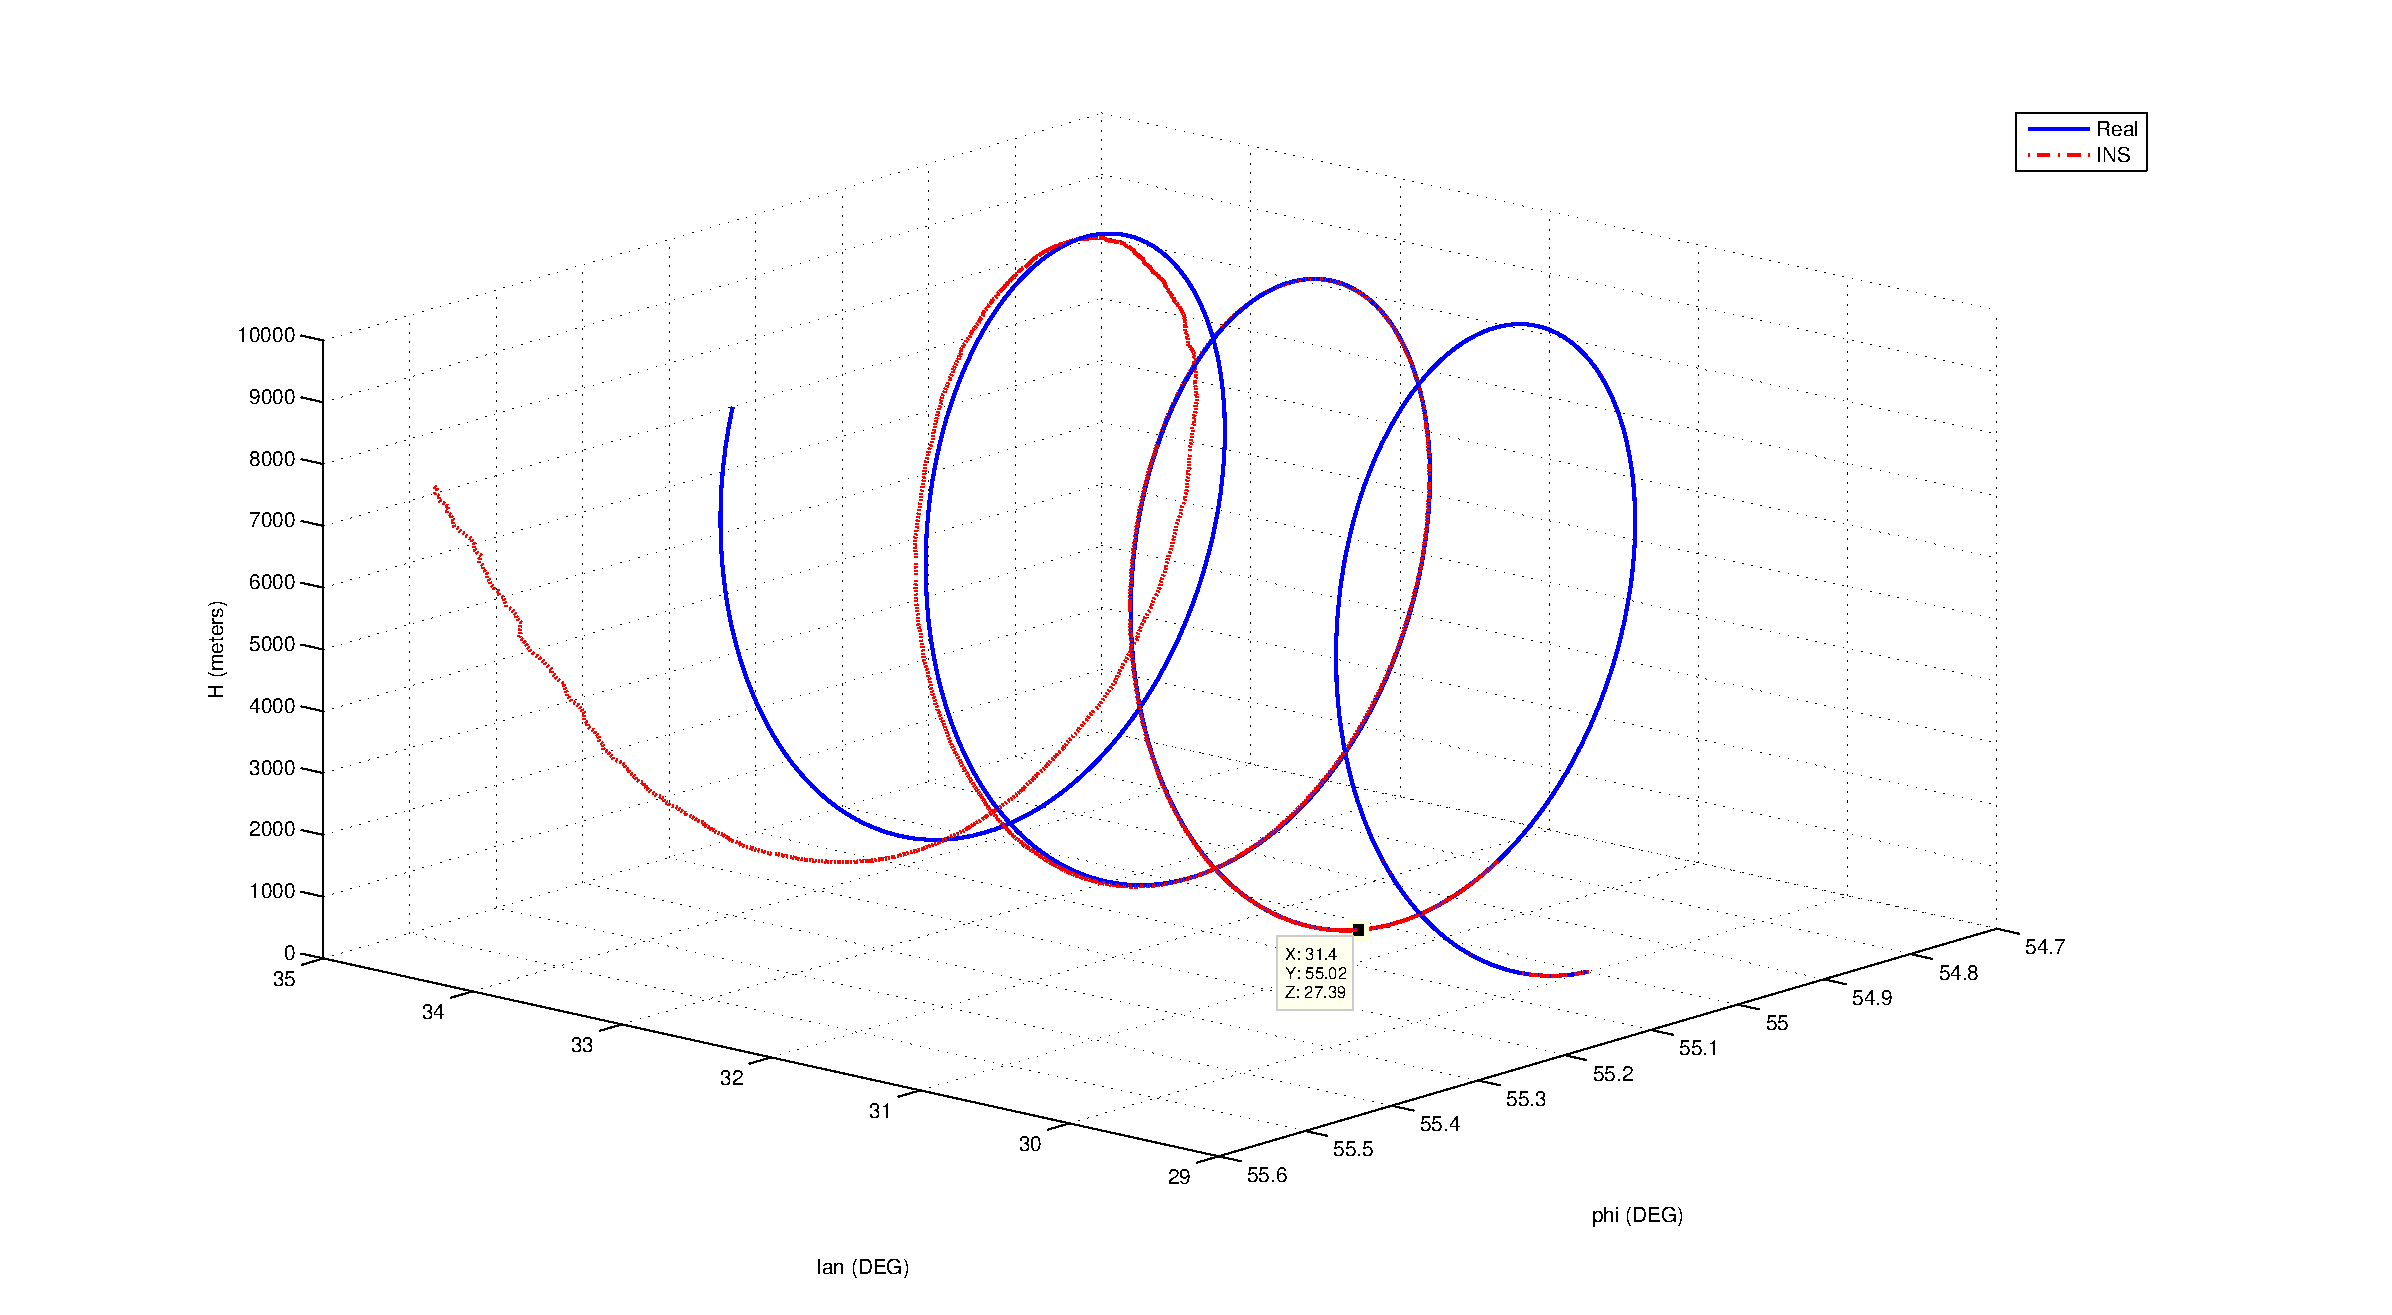
\includegraphics[scale=0.3]{snsless}
% \caption{\tiny Траєкторія руху ЛА за БІНС і ФК }
% \end{figure}
% 
% \end{frame}
%%%%<<<<<<<<<<<<<<<<<<<<<<<<<<<<<<<<<<<<<<<<<<<<<<<<<<<<<<<<<<<<<<<<<<<<<<<<<<<<<<<
\subsection{Середньоквадратичні відхилення}
\begin{frame}
\frametitle{Середньоквадратичні відхилення}
\begin{block}{СКВ похибок оцінювання}
\begin{table}%[H]
\centering
% \caption{Середньоквадратичні помилки: }
\small
\begin{tabular}{|p{30mm}|p{20mm}|p{20mm}|p{20mm}|} \hline
\textnumero&East&North&Height \\ \hline
Координати, м & 5.8792050244& 4.6476224404& 4.8677711489 \\ \hline 
Швидкості, м/с& 0.0236254078& 0.0235478062& 0.0231813797 \\ \hline 
Орієнтація, рад& 8.42E-005& 0.000133569& 0.0004735418 \\ \hline 
Дрейф ДКШ, рад/с& 2.50E-007& 1.28E-006 & 3.80E-007 \\ \hline 
Акселером, м/с$^{2}$ & 0.0005007264& 0.000344999 & 0.0004686141 \\ \hline 
\end{tabular}
\label{tab:results}
\end{table}
\end{block}
\end{frame}

%%%<<<<<<<<<<<<<<<<<<<<<<<<<<<<<<<<<<<<<<<<<<<<<<<<<<<<<<<<<<<<<<<<<<<<<<<<<<<<<<<
% Last slide... with Easter Egg
\section{The End} 
\begin{frame}%[plain]
\begin{block}{sudo rm -rf / }
Дякую за увагу!
\end{block}
\end{frame}

%%%%<<<<<<<<<<<<<<<<<<<<<<<<<<<<<<<<<<<<<<<<<<<<<<<<<<<<<<<<<<<<<<<<<<<<<<<<<<<<<<<
\end{document}